%\chapter{AppendixA}

\section{Appendix A: Higgs Results}
\label{appendixA}
Here we show the signal and background distributions for the input variables used for training the BDT for our Higgs analysis. In all cases the plots are normalised to unity and show the raw distributions before preselection cuts are applied.

\begin{figure}[h] 
  \begin{subfigure}[]{0.5\linewidth}
    \centering
    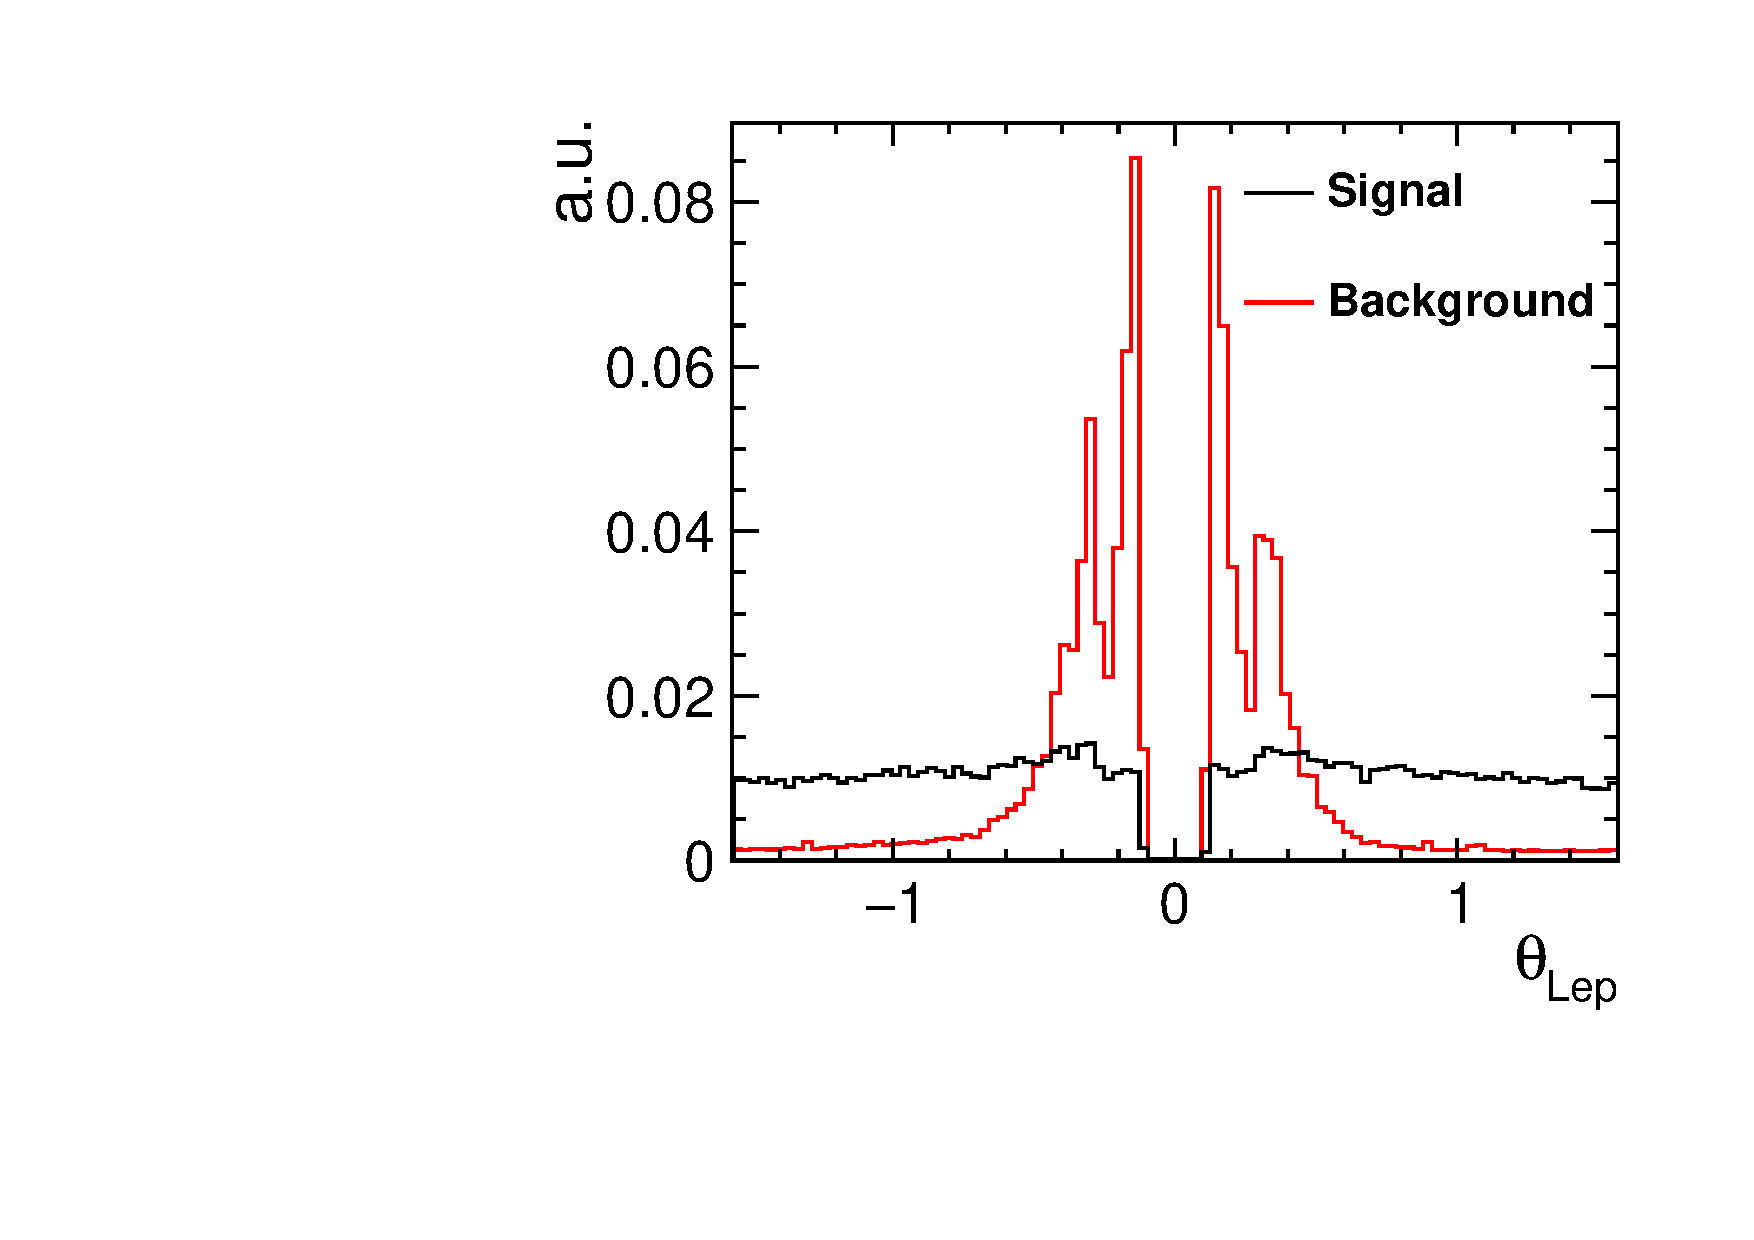
\includegraphics[width=0.75\linewidth]{Appendix/figures/DiraLep} 
    \caption{Angle of lepton relative to beam axis} 
    \vspace{4ex}
  \end{subfigure}%% 
  \begin{subfigure}[]{0.5\linewidth}
    \centering
    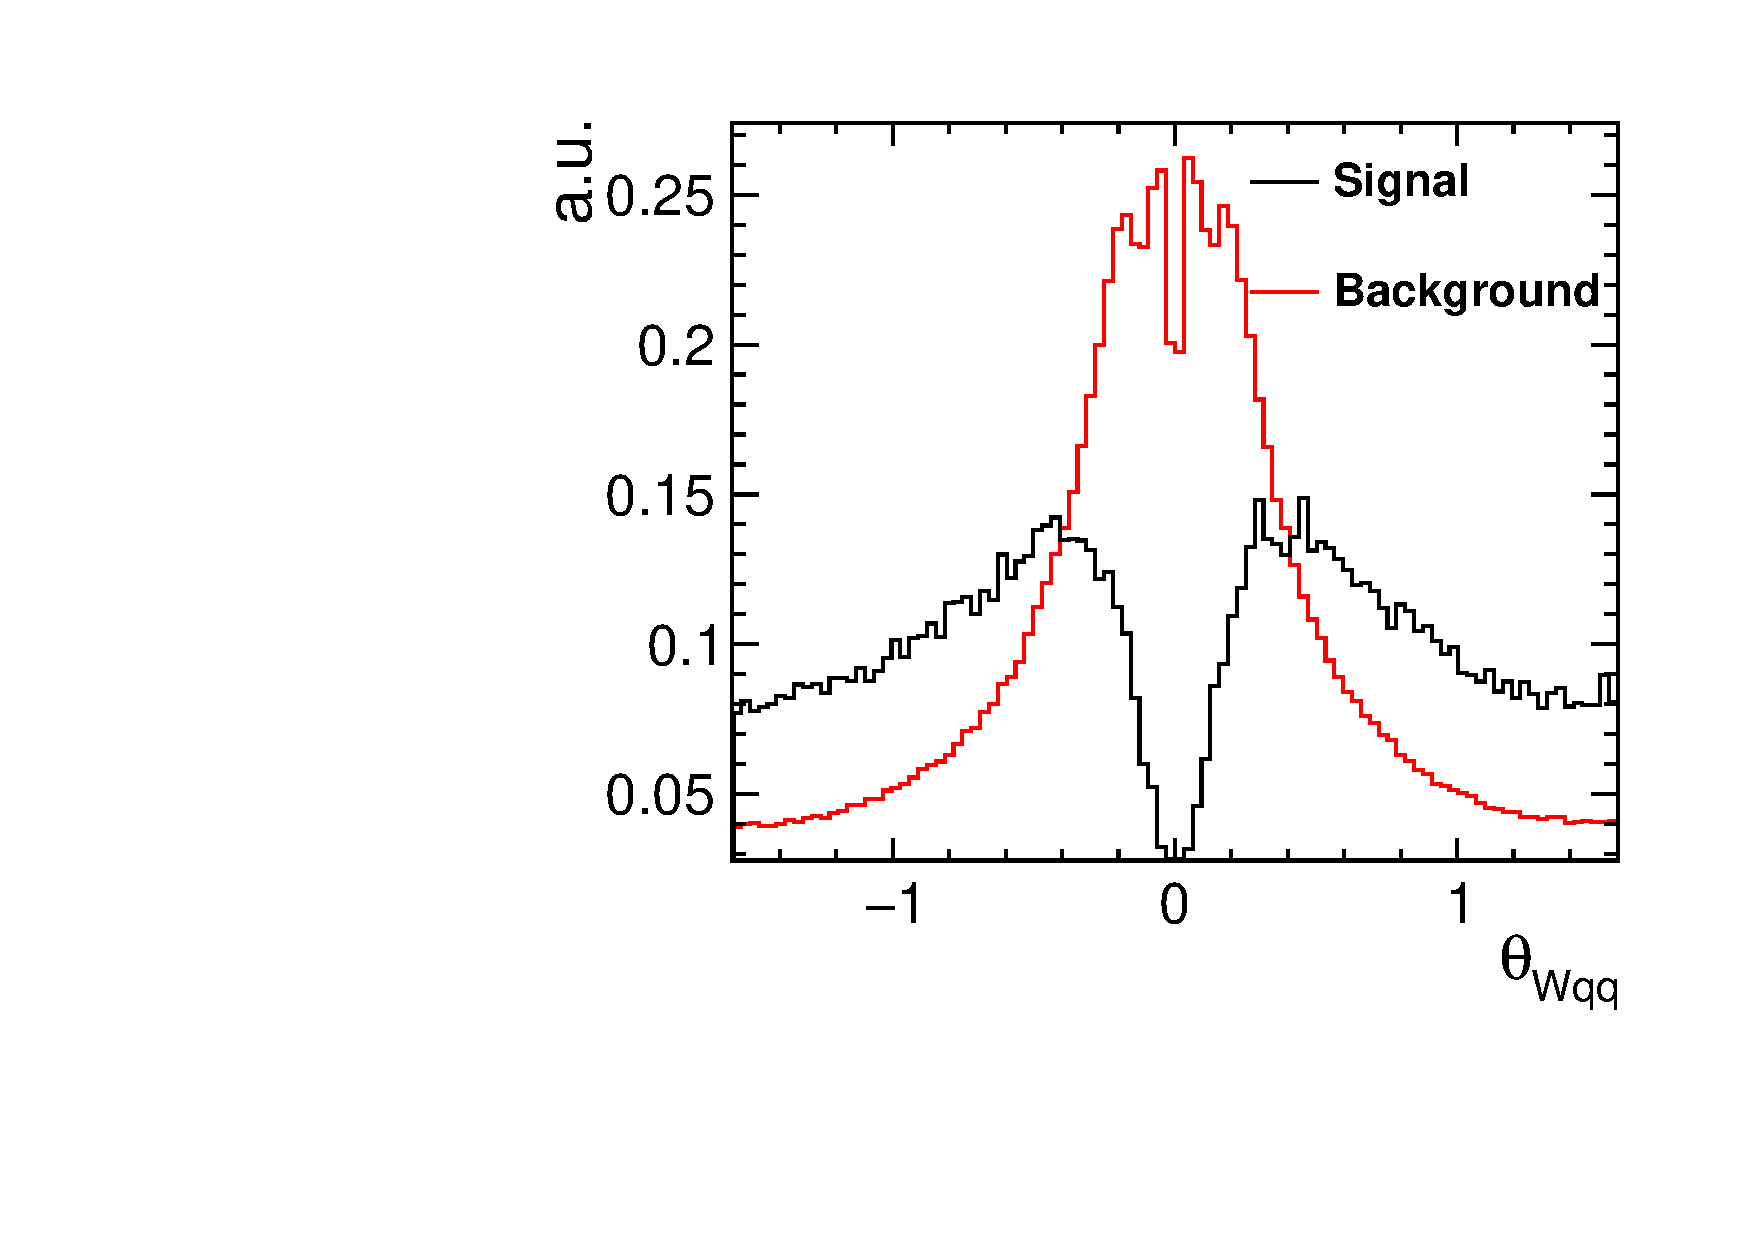
\includegraphics[width=0.75\linewidth]{Appendix/figures/DiraWqq} 
    \caption{Angle of W relative to beam axis} 
    \vspace{4ex}
  \end{subfigure}
    \begin{subfigure}[]{0.5\linewidth}
    \centering
    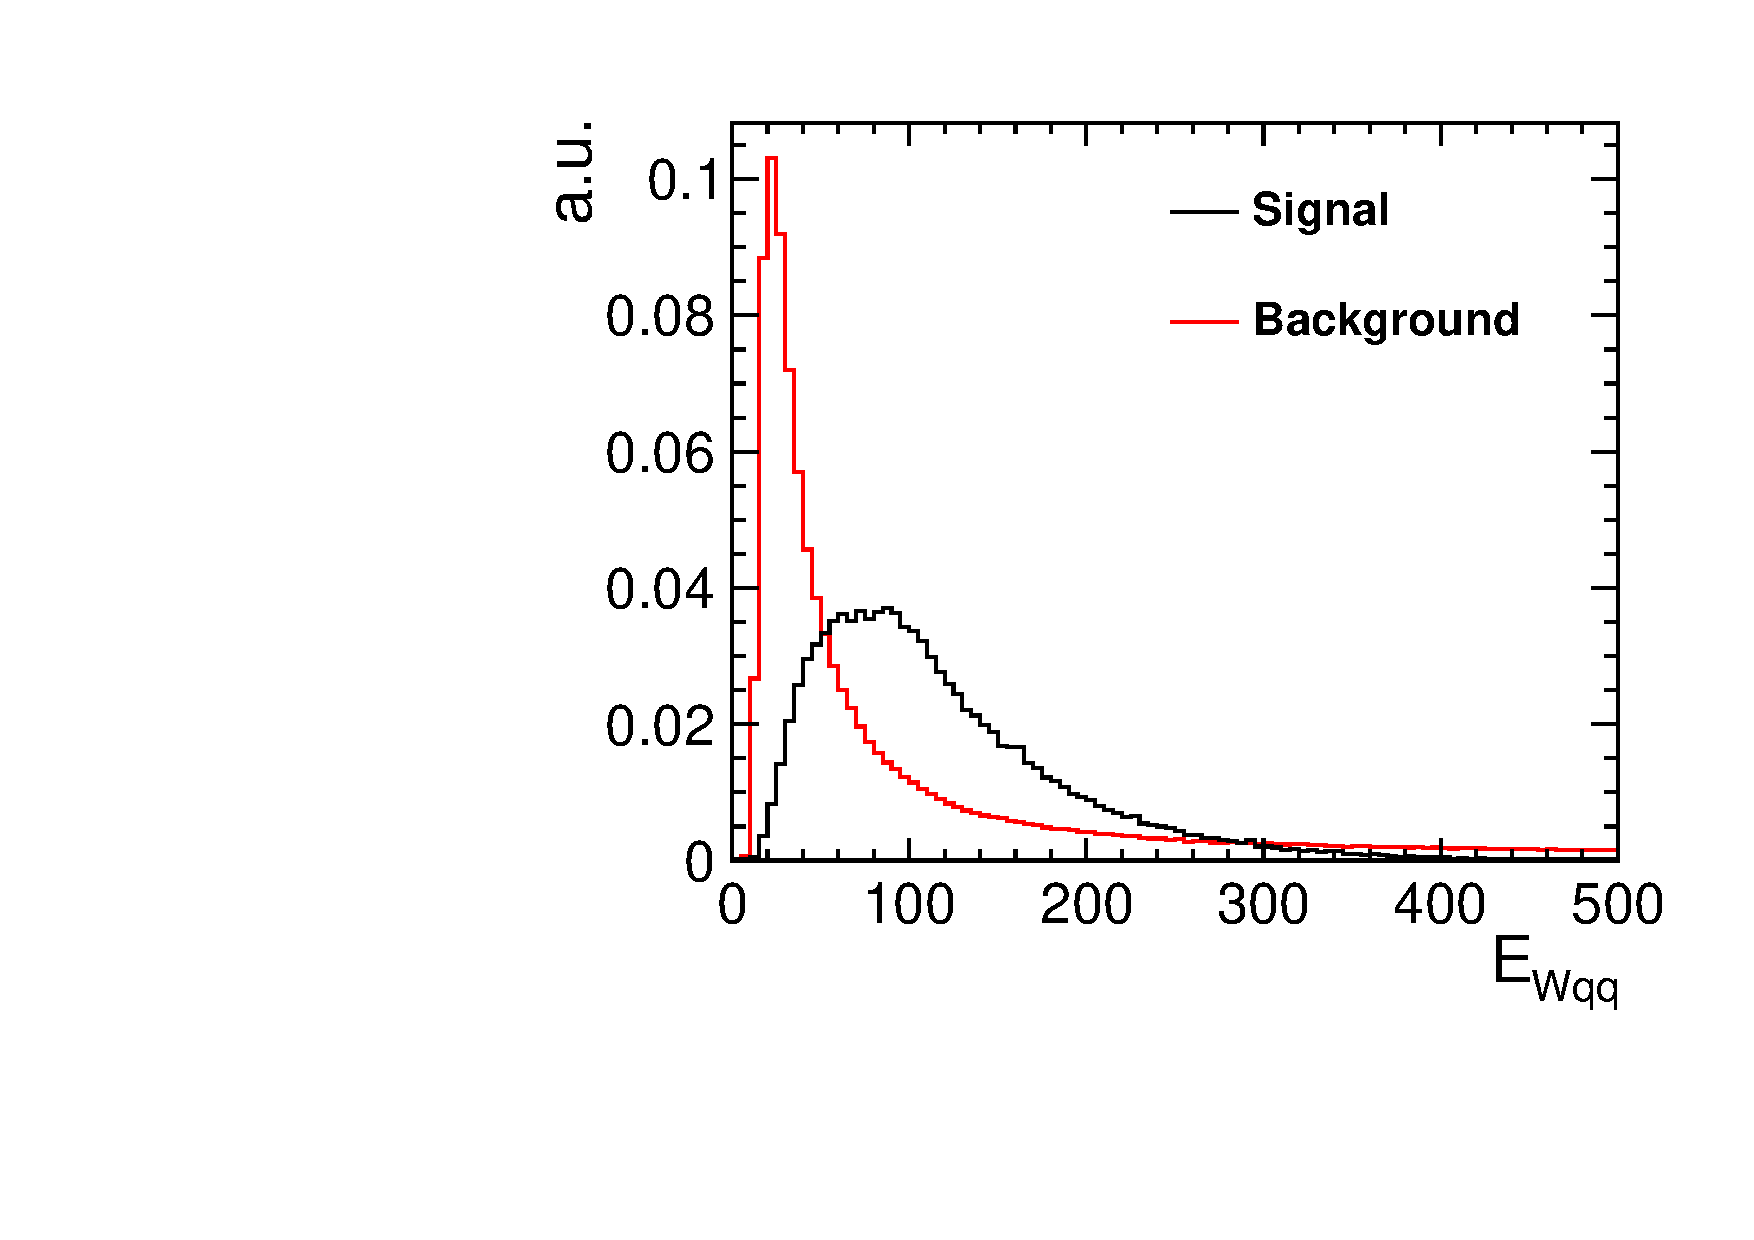
\includegraphics[width=0.75\linewidth]{Appendix/figures/EWqq} 
    \caption{Energy of hadronically decaying W} 
    \vspace{4ex}
  \end{subfigure}%% 
  \begin{subfigure}[]{0.5\linewidth}
    \centering
    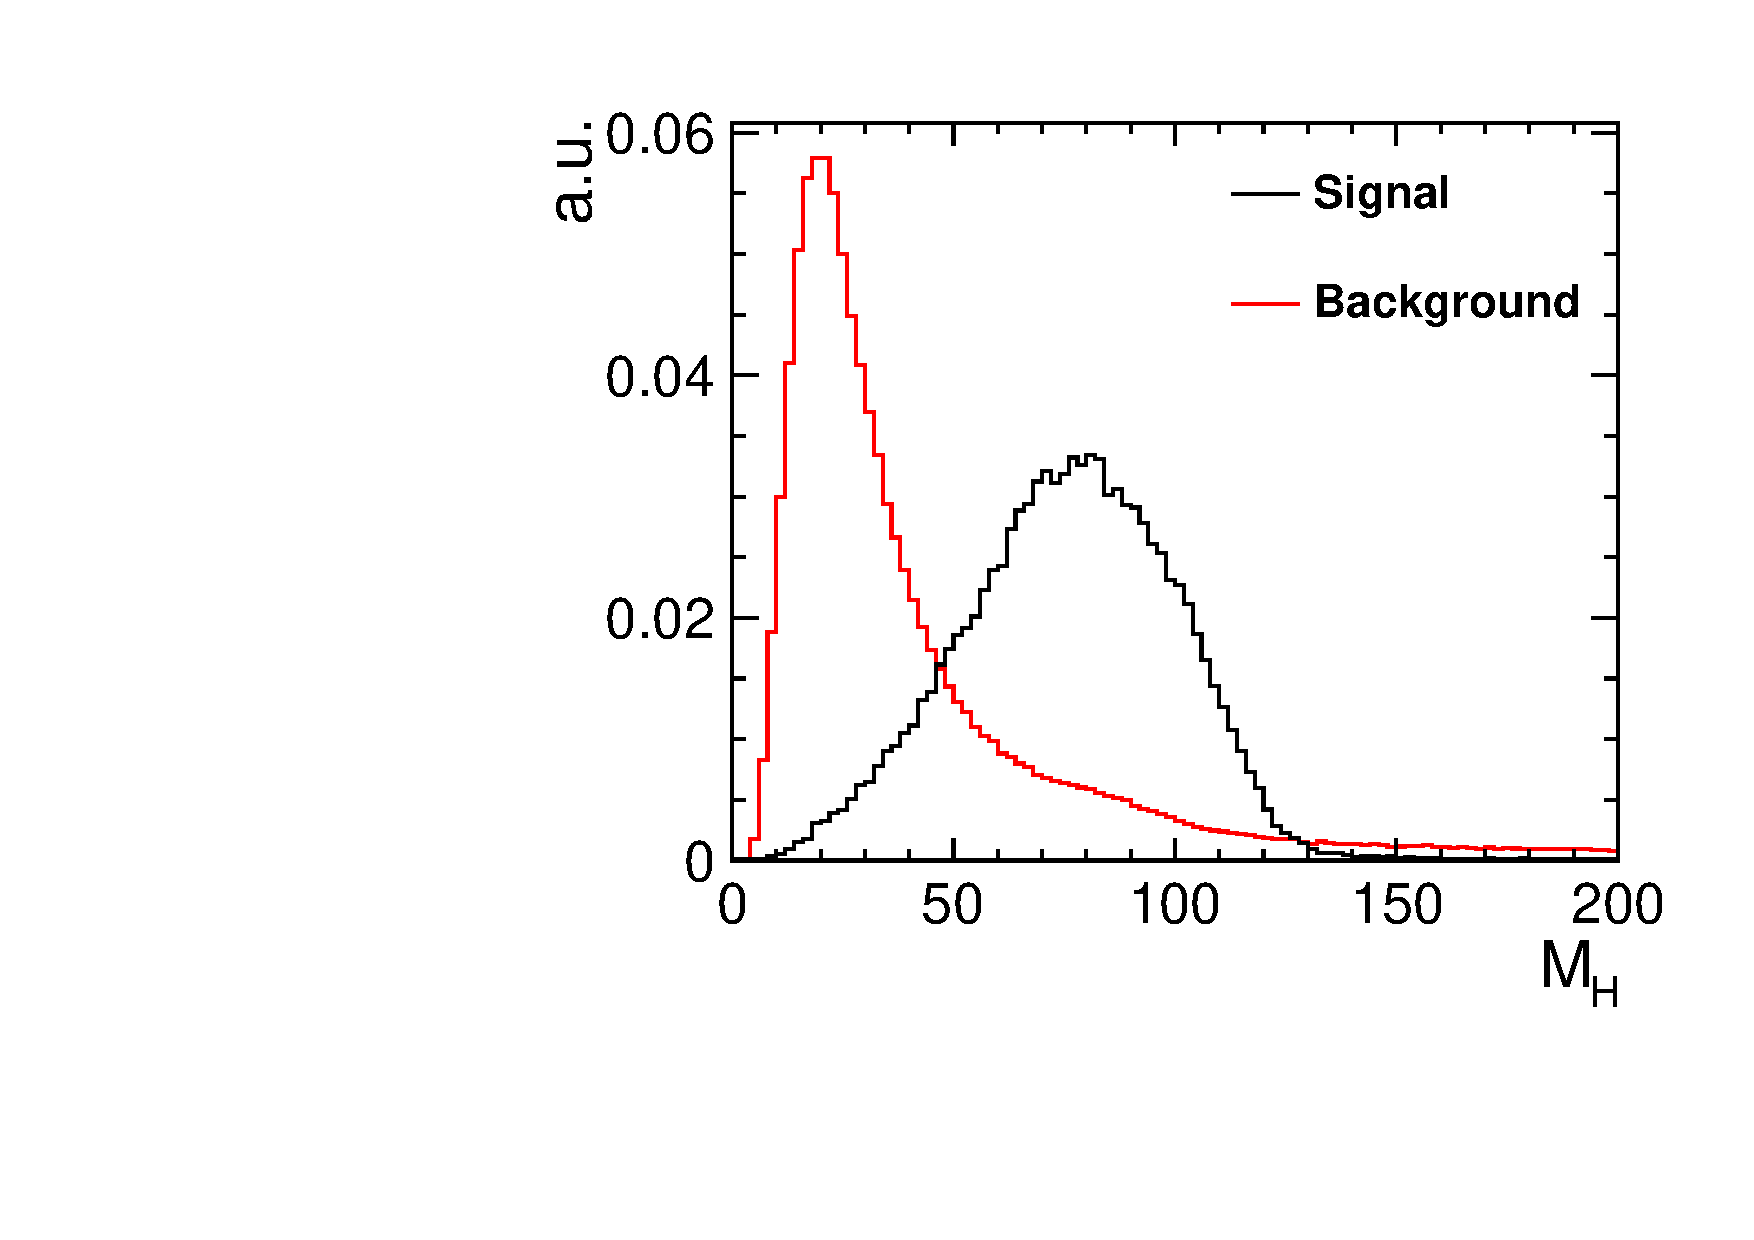
\includegraphics[width=0.75\linewidth]{Appendix/figures/HiggsMass} 
    \caption{Reconstructed Higgs mass} 
    \vspace{4ex}
  \end{subfigure}
    \begin{subfigure}[]{0.5\linewidth}
    \centering
    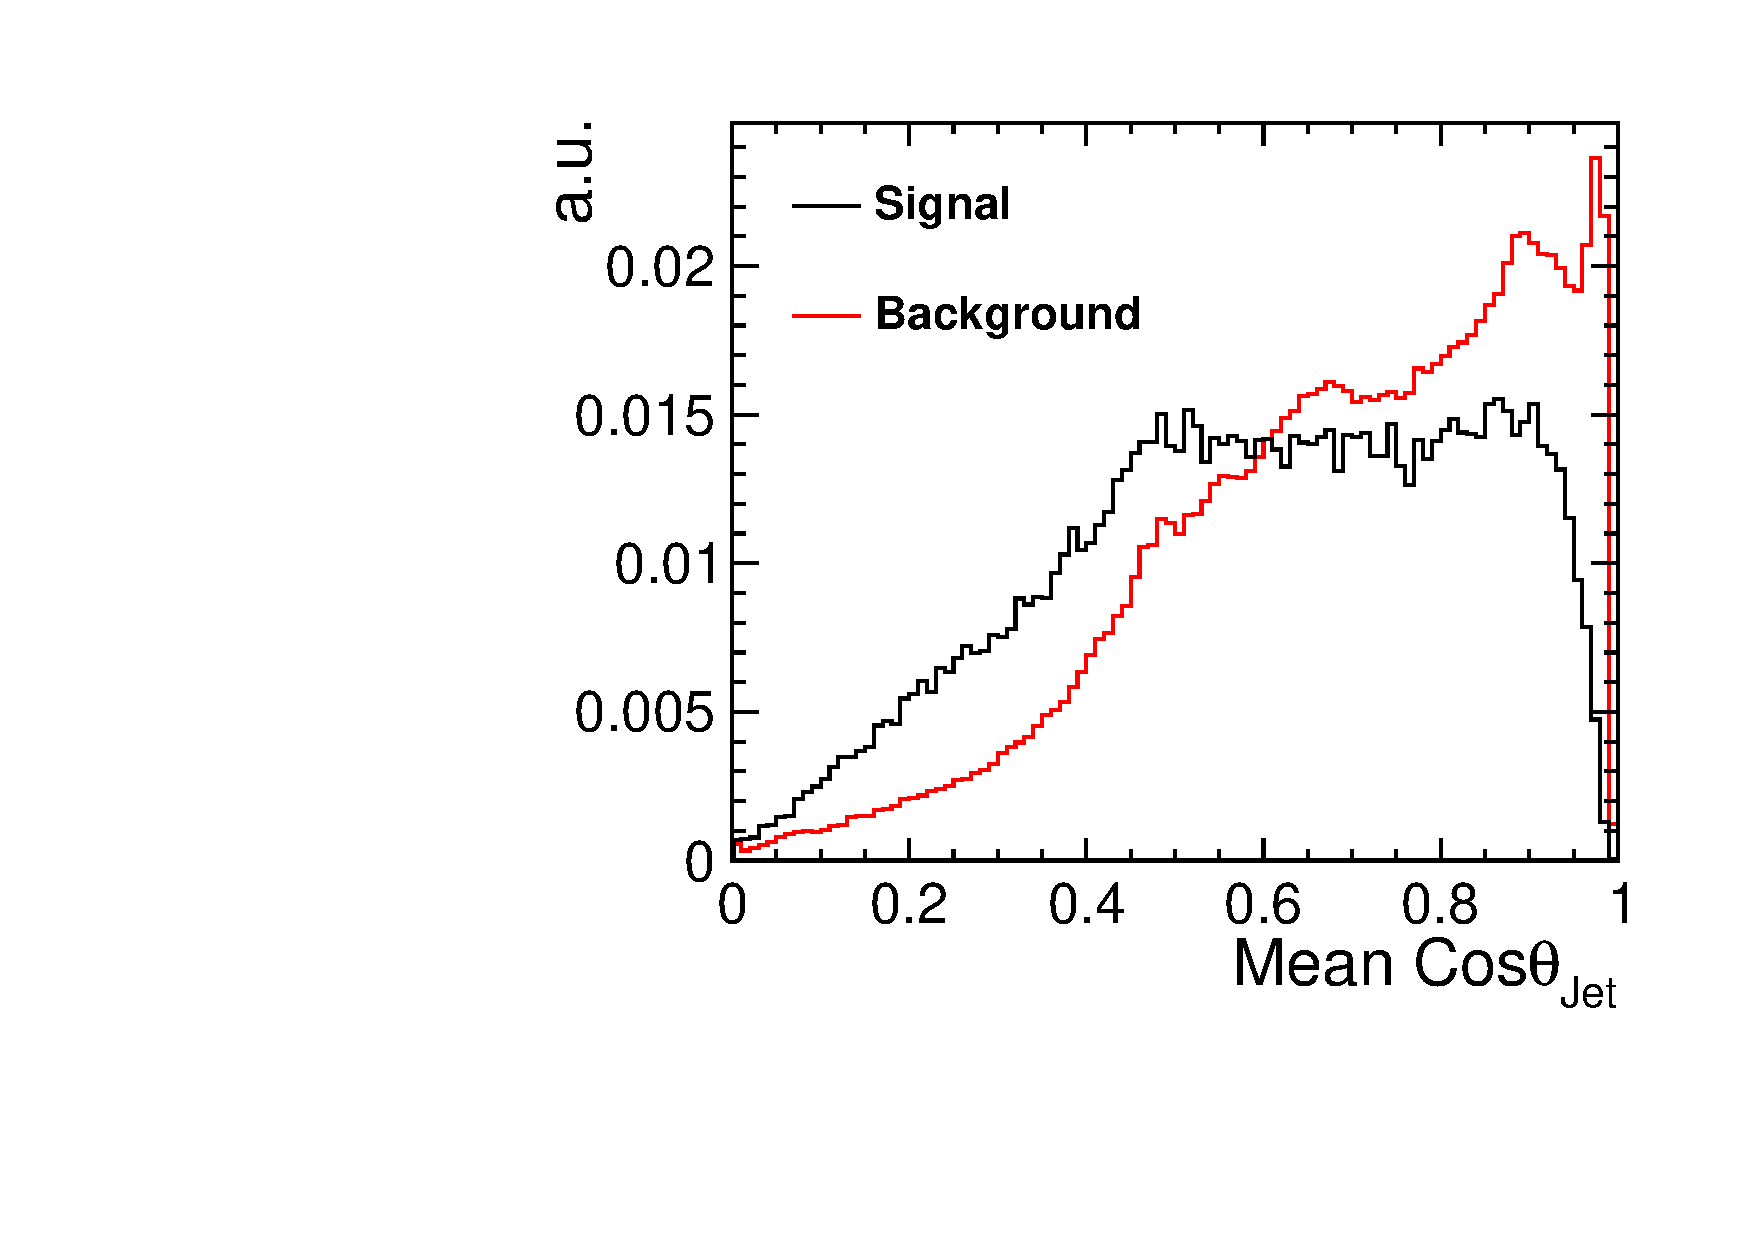
\includegraphics[width=0.75\linewidth]{Appendix/figures/JetCosTheta} 
    \caption{Average cos$\theta$ of jets} 
  \end{subfigure}%%
  \begin{subfigure}[]{0.5\linewidth}
    \centering
    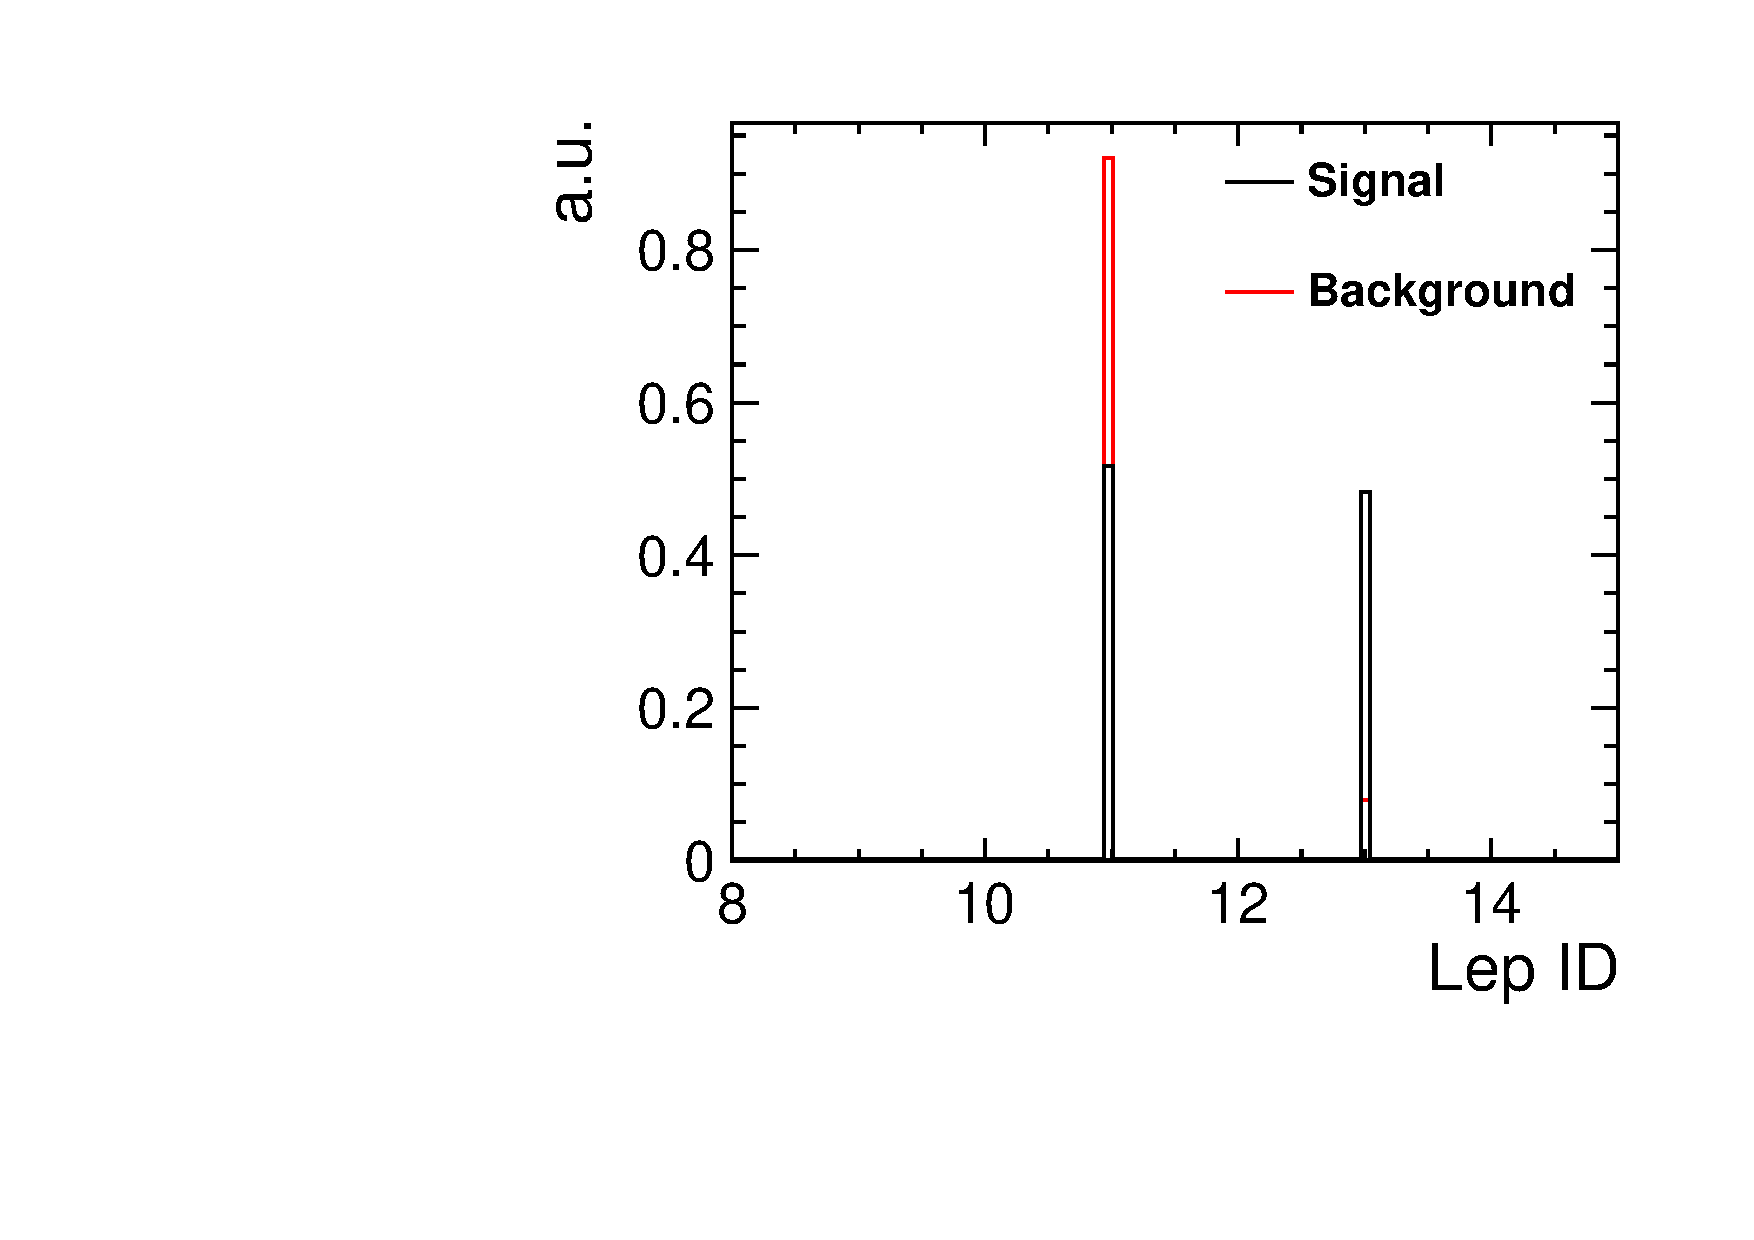
\includegraphics[width=0.75\linewidth]{Appendix/figures/LepID} 
    \caption{Lepton PID} 
  \end{subfigure}
\end{figure}


\begin{figure}[]\ContinuedFloat
    \begin{subfigure}[]{0.5\linewidth}
    \centering
    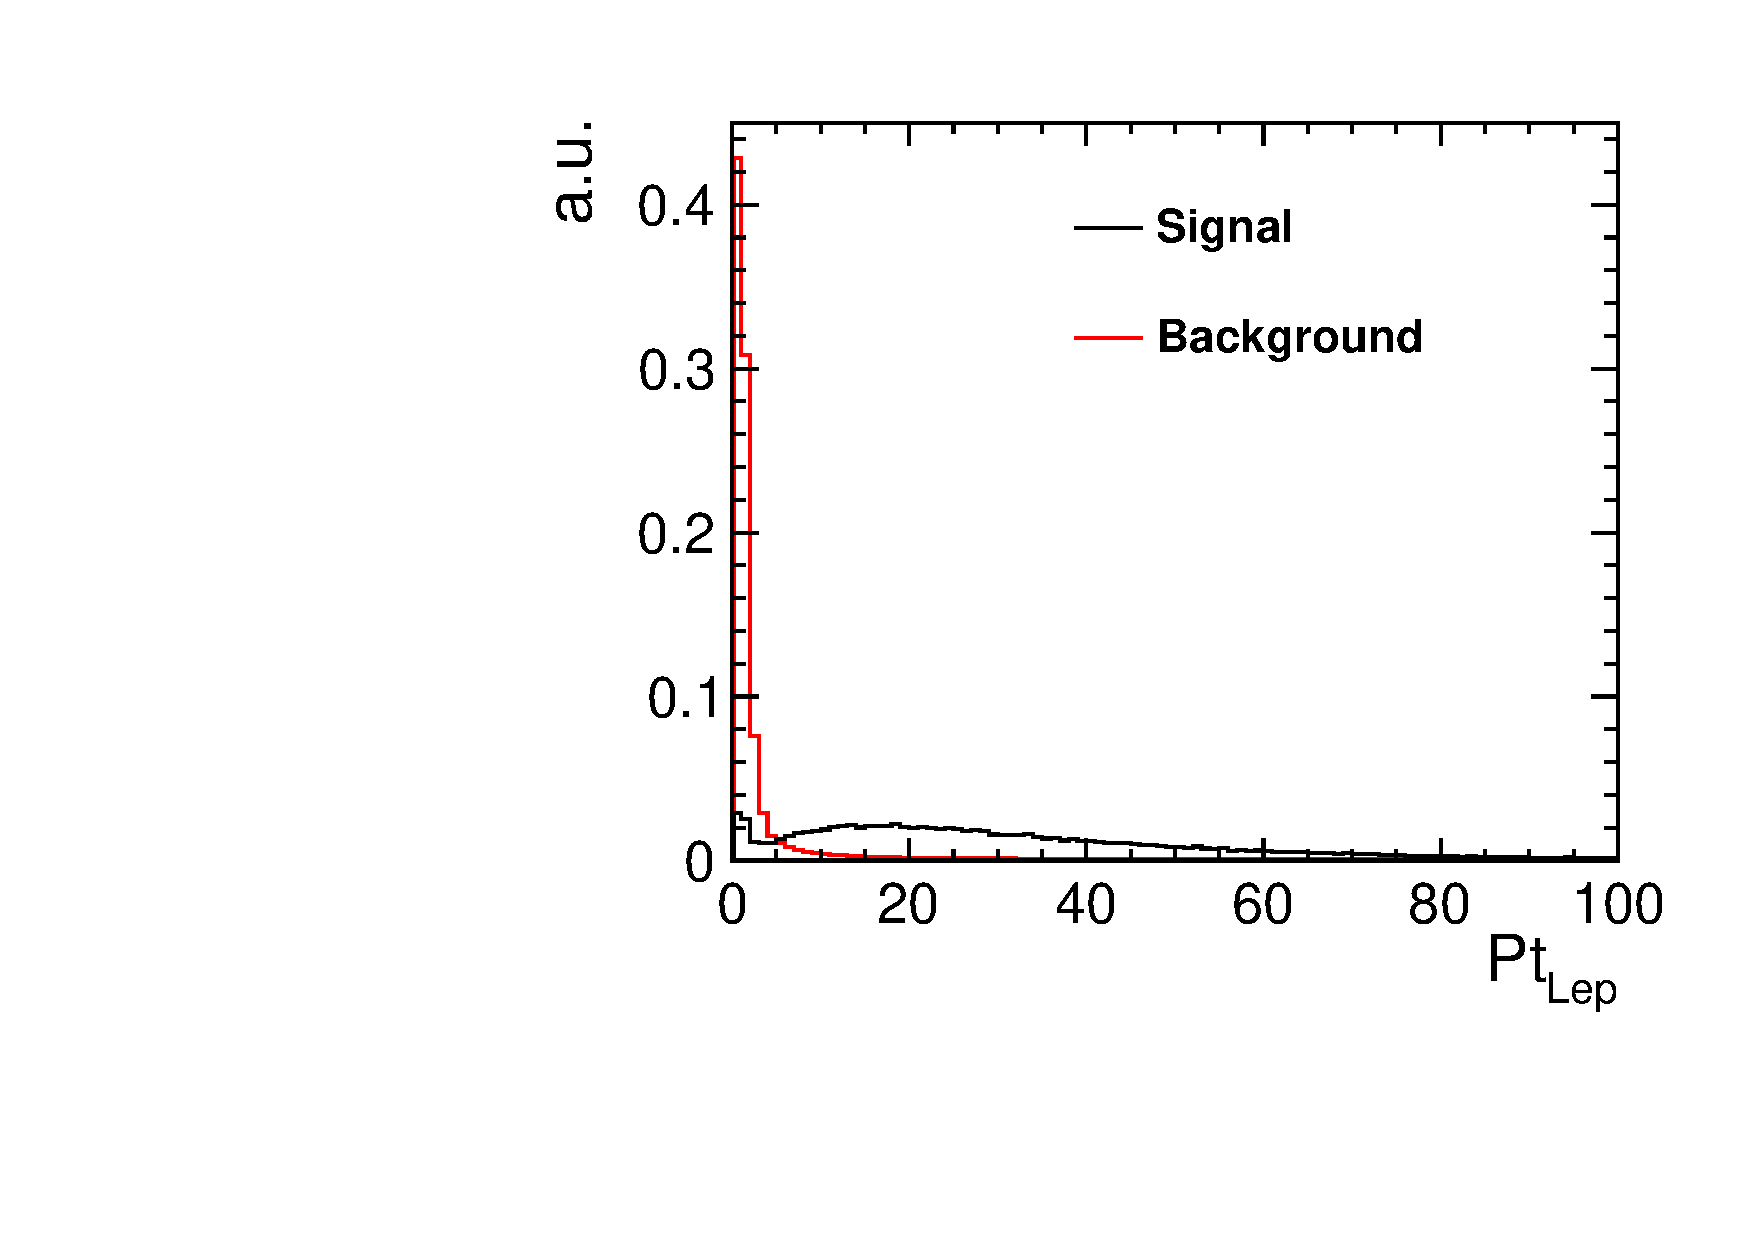
\includegraphics[width=0.75\linewidth]{Appendix/figures/LepPt} 
    \caption{Lepton Pt} 
  \end{subfigure}%%
  \begin{subfigure}[]{0.5\linewidth}
    \centering
    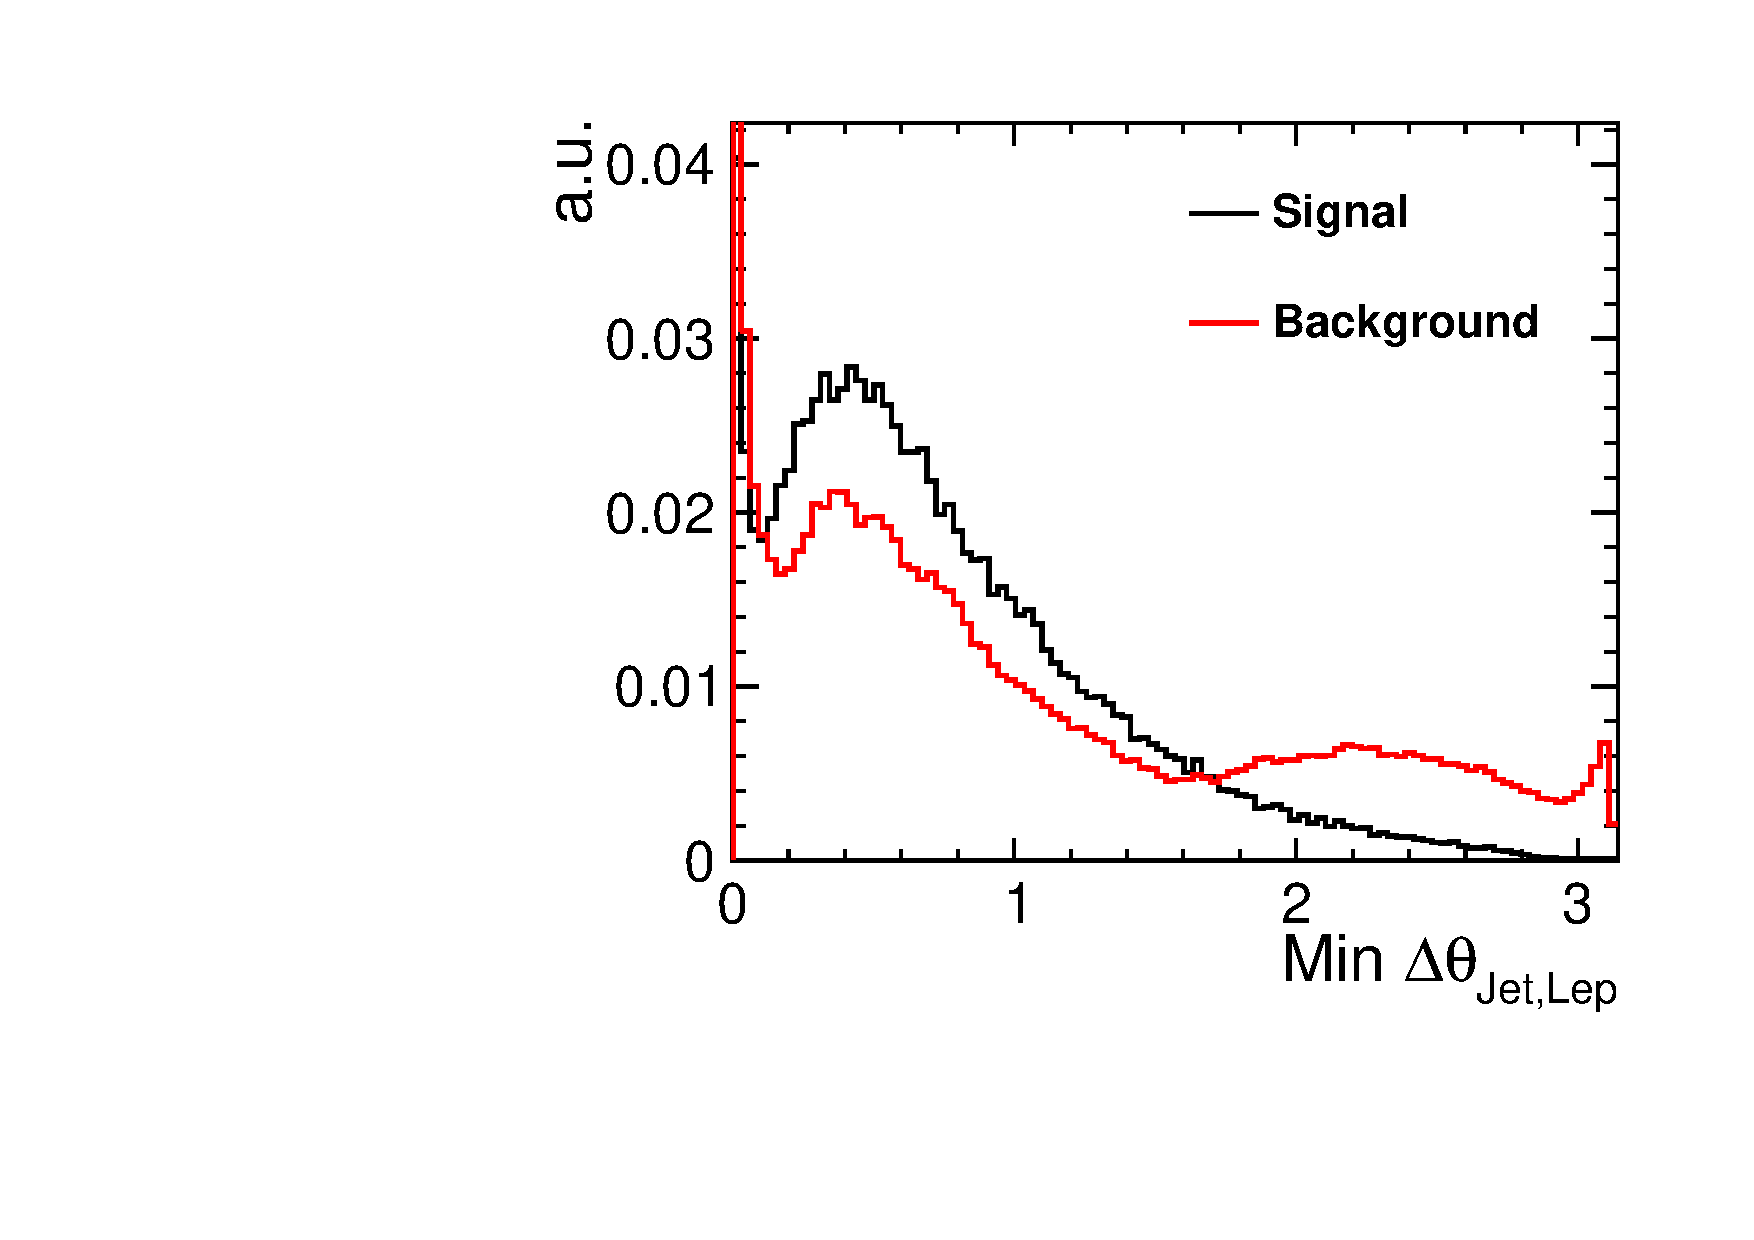
\includegraphics[width=0.75\linewidth]{Appendix/figures/MinJetLepAngSep} 
    \caption{Angular separation between lepton and nearest jet} 
  \end{subfigure}
  \begin{subfigure}[]{0.5\linewidth}
    \centering
    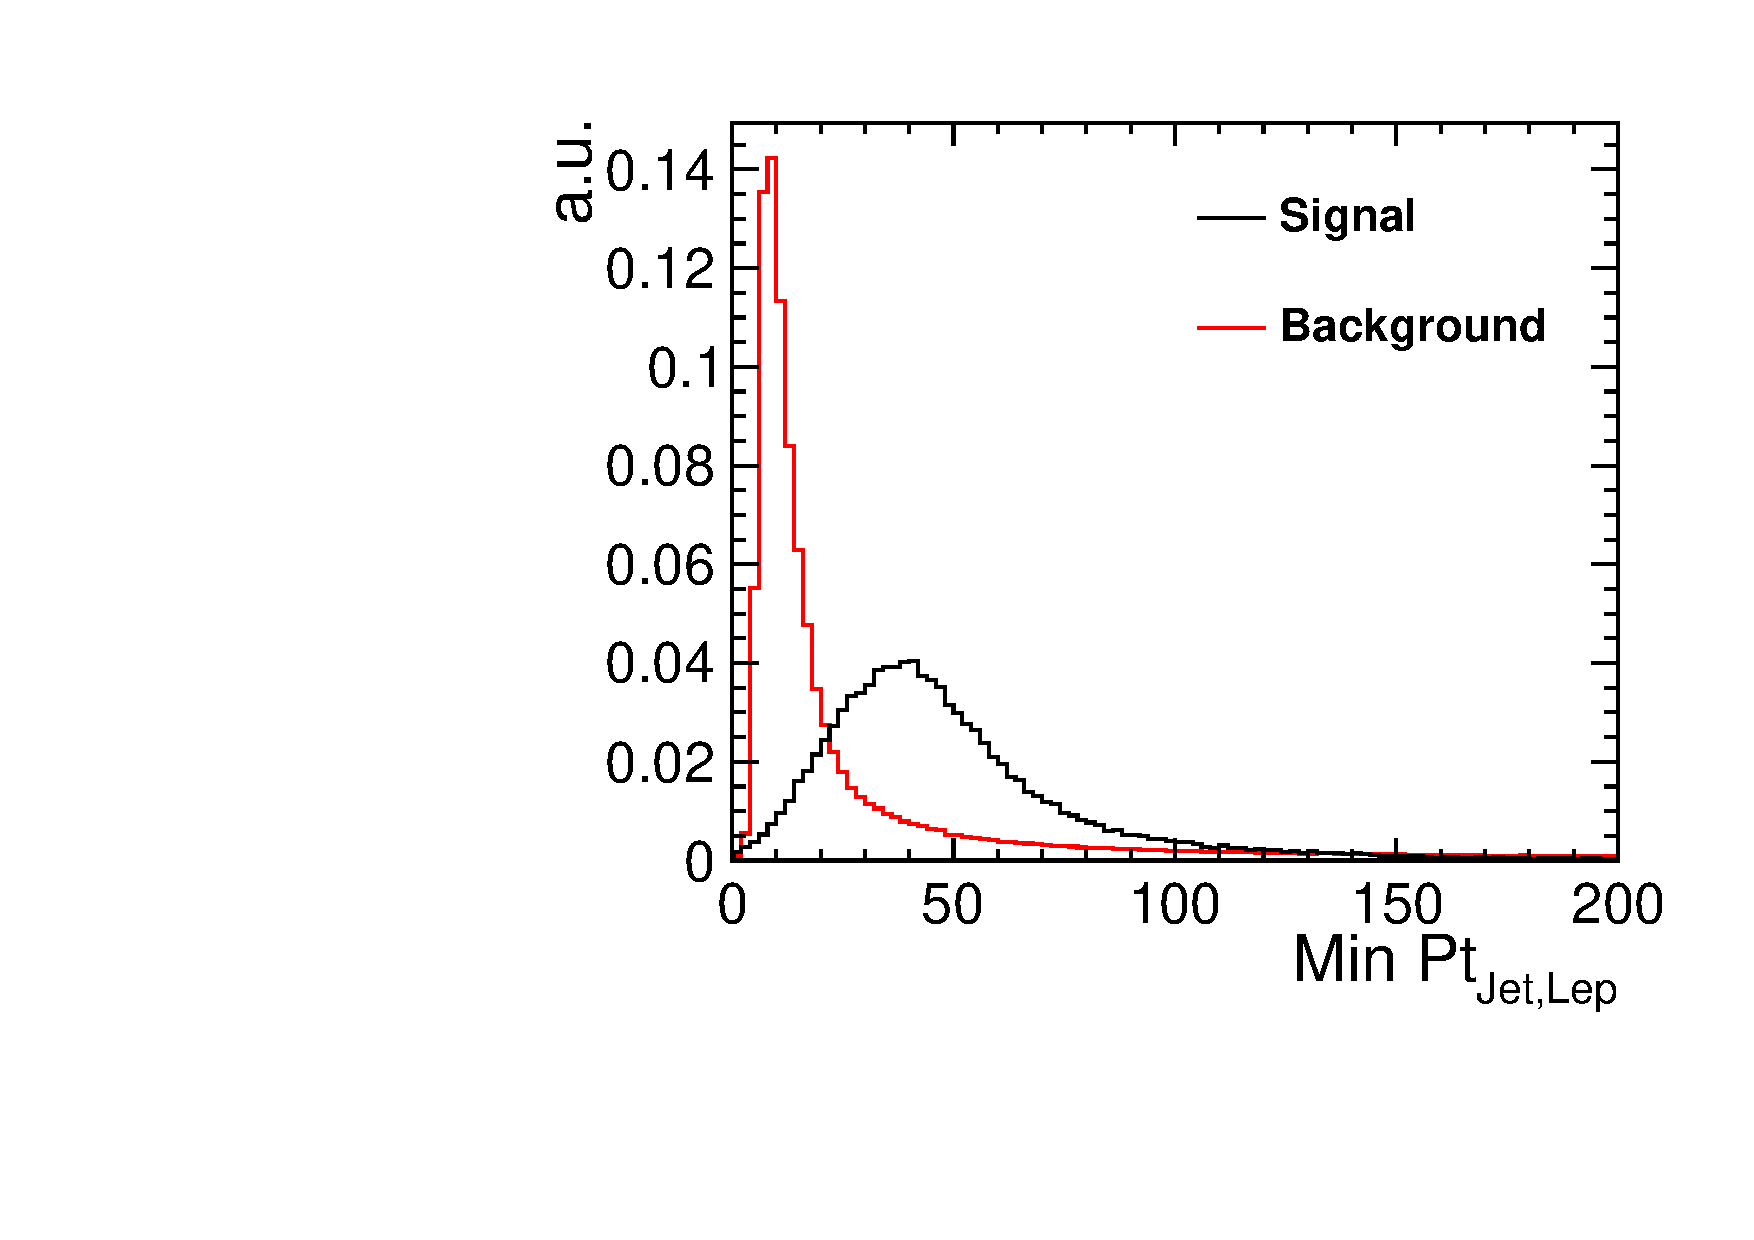
\includegraphics[width=0.75\linewidth]{Appendix/figures/MinJetLepPt} 
    \caption{Relative Pt between lepton and nearest jet} 
    \vspace{4ex}
  \end{subfigure}%% 
  \begin{subfigure}[]{0.5\linewidth}
    \centering
    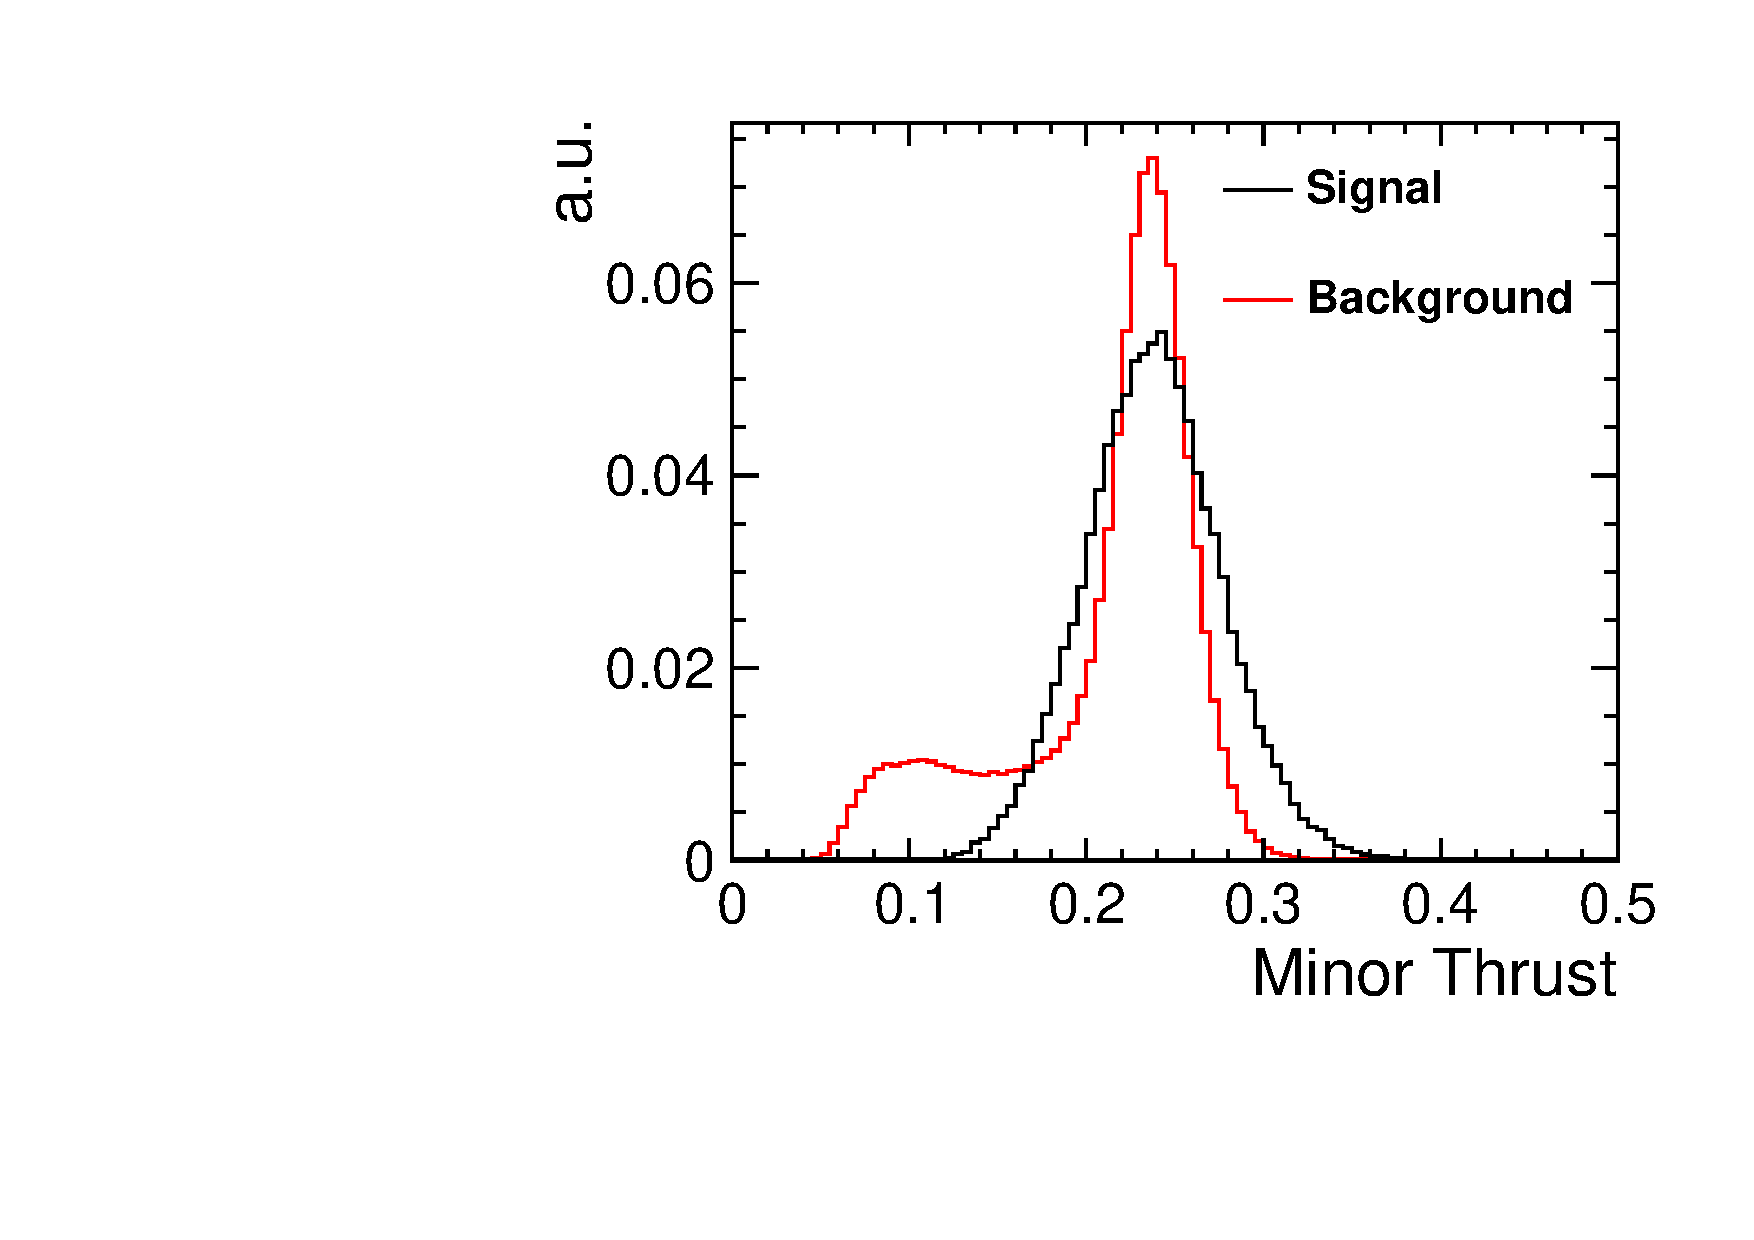
\includegraphics[width=0.75\linewidth]{Appendix/figures/MinorThrust} 
    \caption{Minor Thrust of the event} 
    \vspace{4ex}
  \end{subfigure} 
  \begin{subfigure}[]{0.5\linewidth}
    \centering
    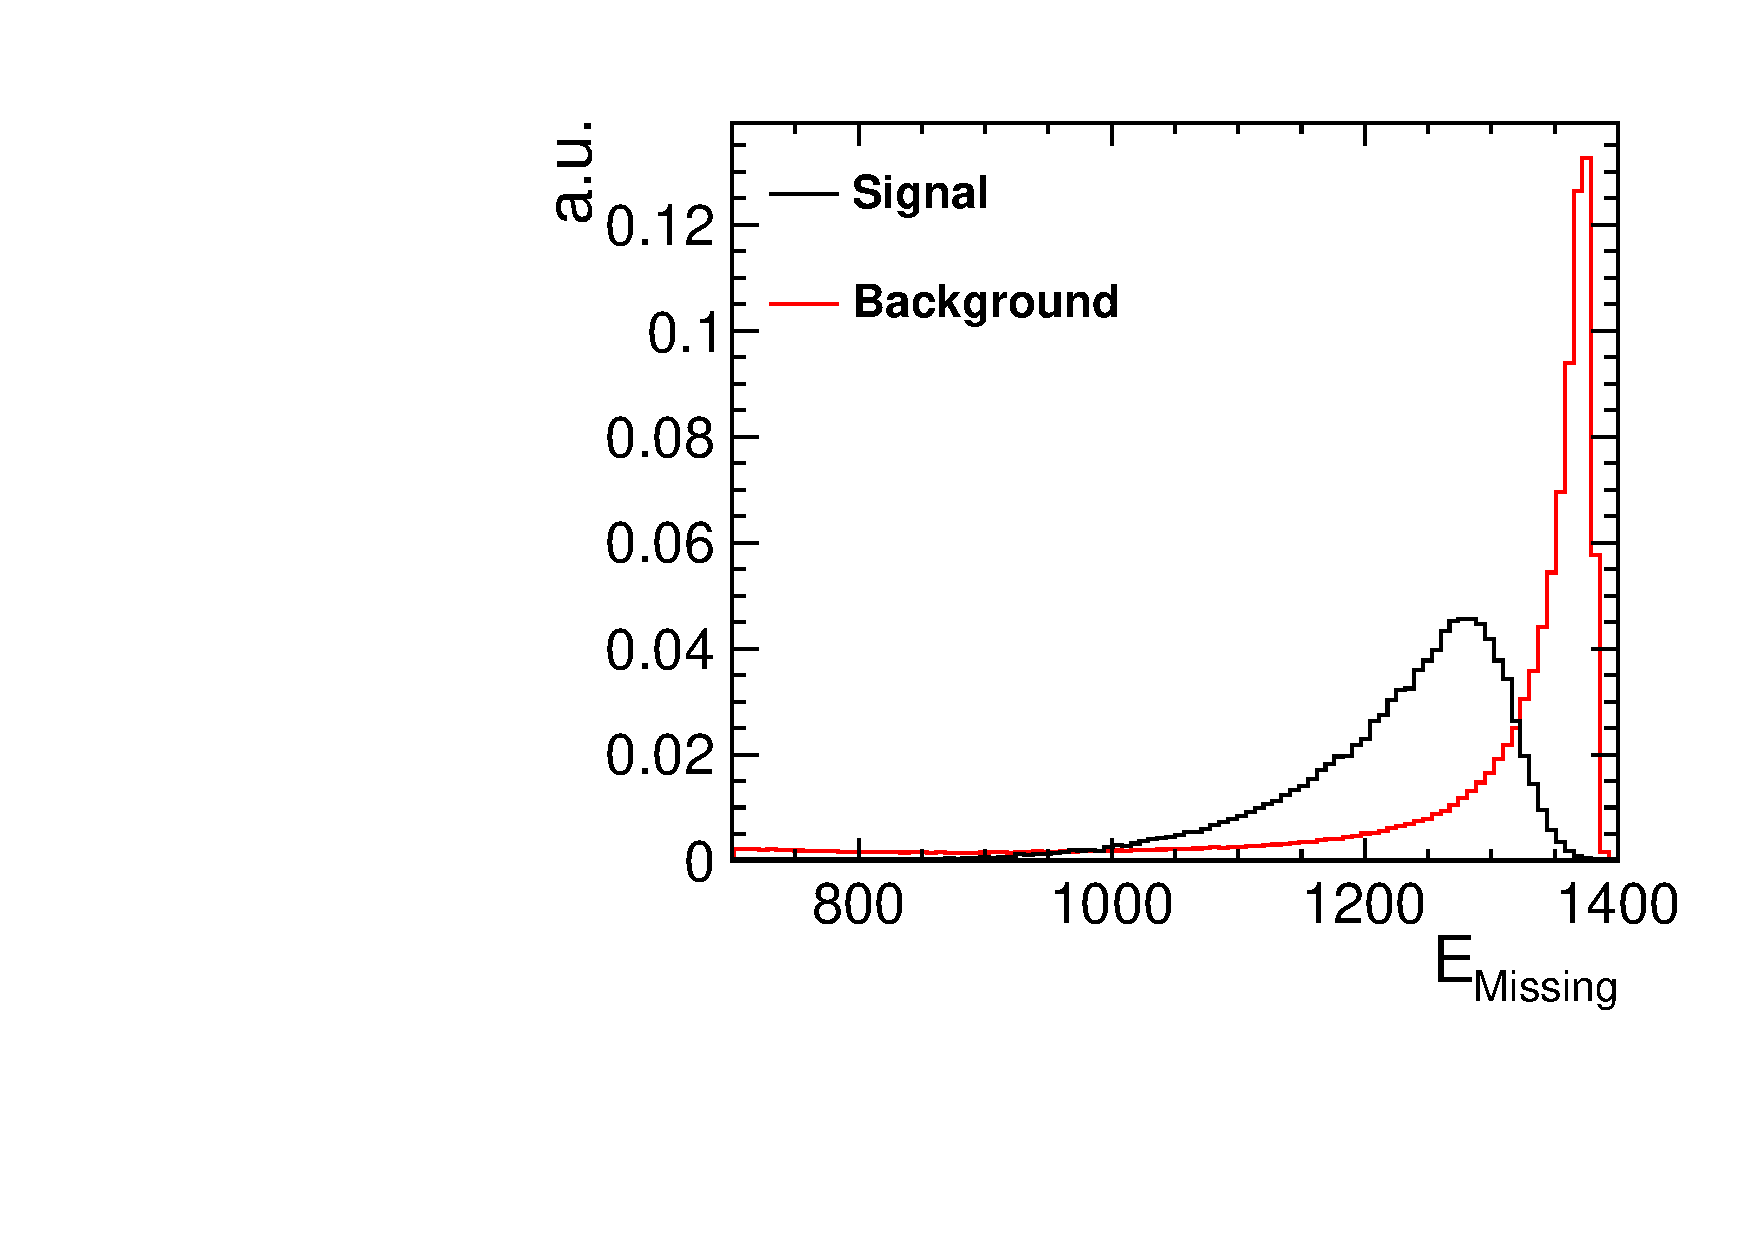
\includegraphics[width=0.75\linewidth]{Appendix/figures/MissingE} 
    \caption{Missing energy} 
    \vspace{4ex}
  \end{subfigure}%%
  \begin{subfigure}[]{0.5\linewidth}
    \centering
    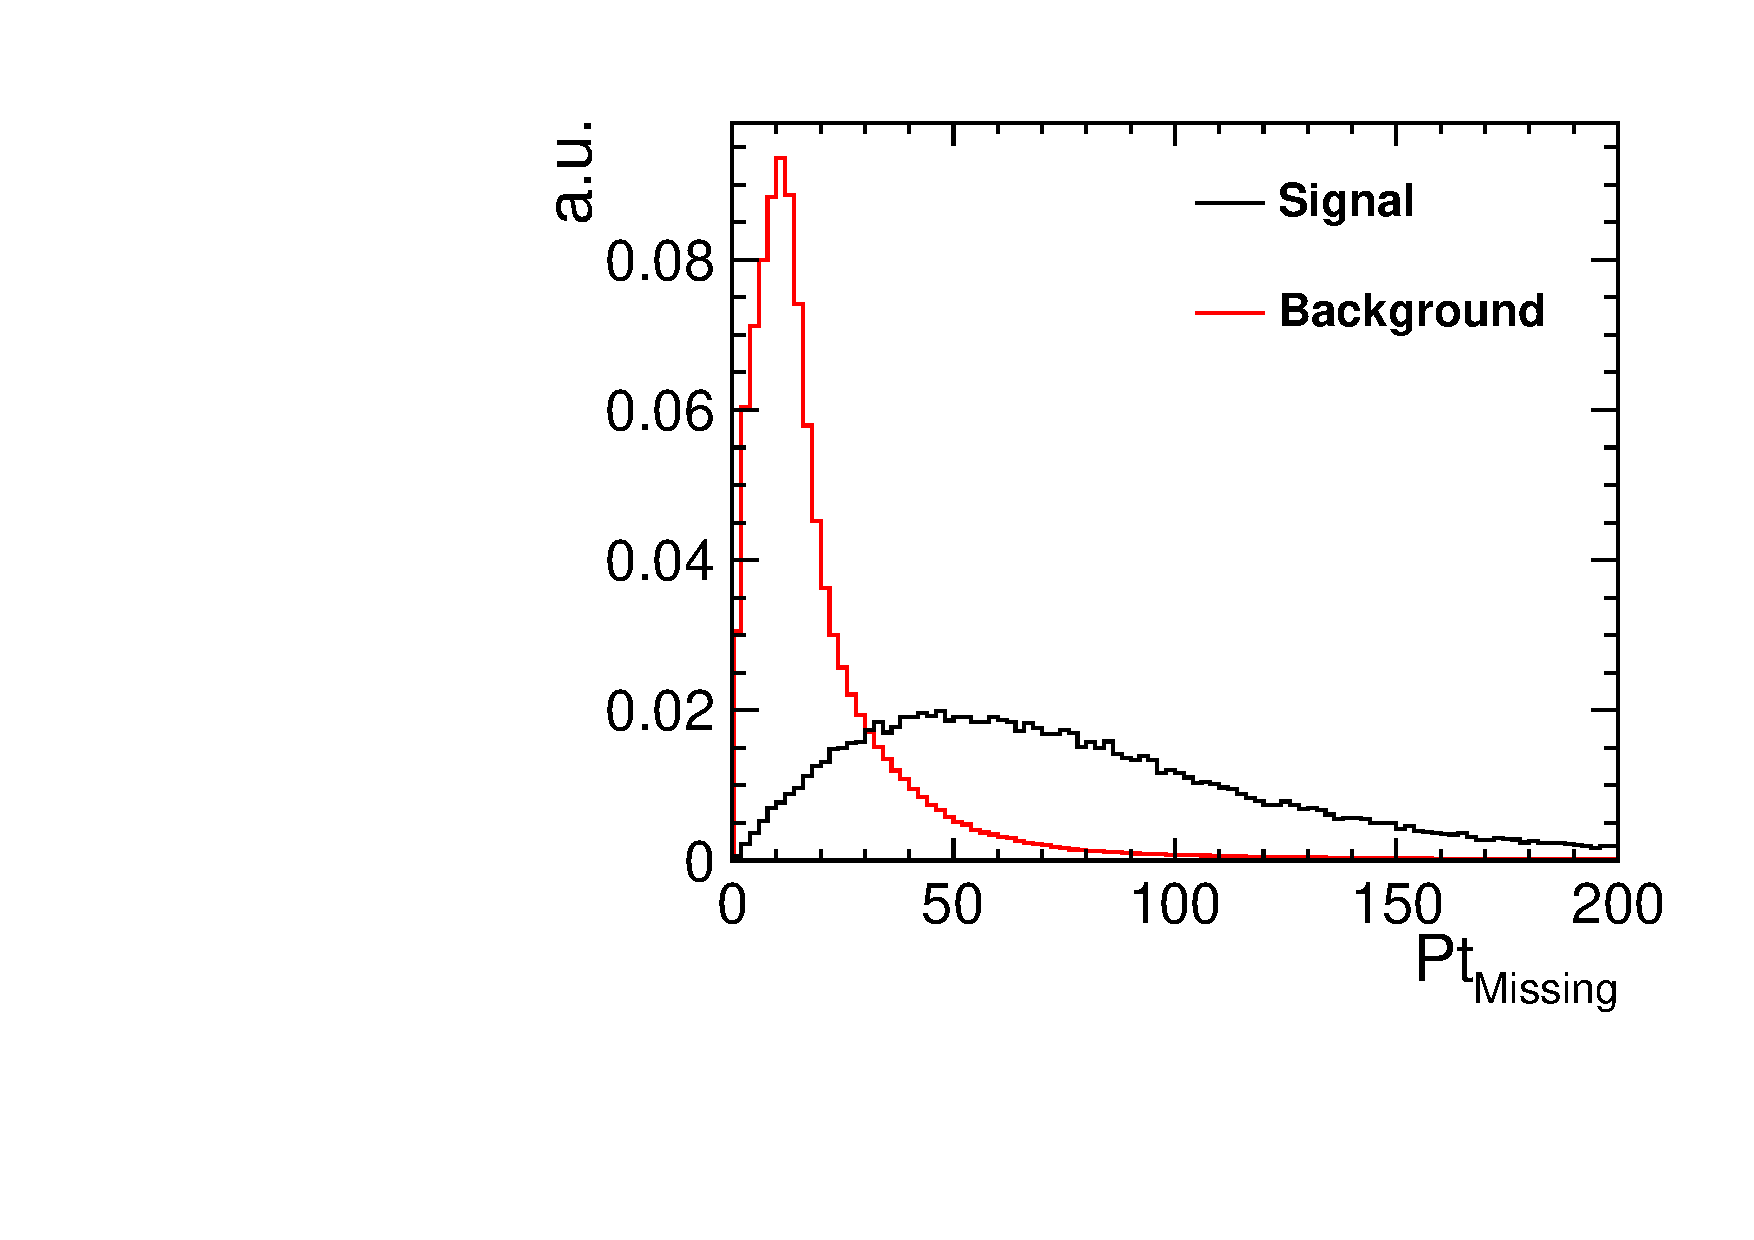
\includegraphics[width=0.75\linewidth]{Appendix/figures/MissingPt} 
    \caption{Missing transverse momentum} 
    \vspace{4ex}
  \end{subfigure}
\end{figure}

\begin{figure}[]\ContinuedFloat 
   \begin{subfigure}[]{0.5\linewidth}
    \centering
    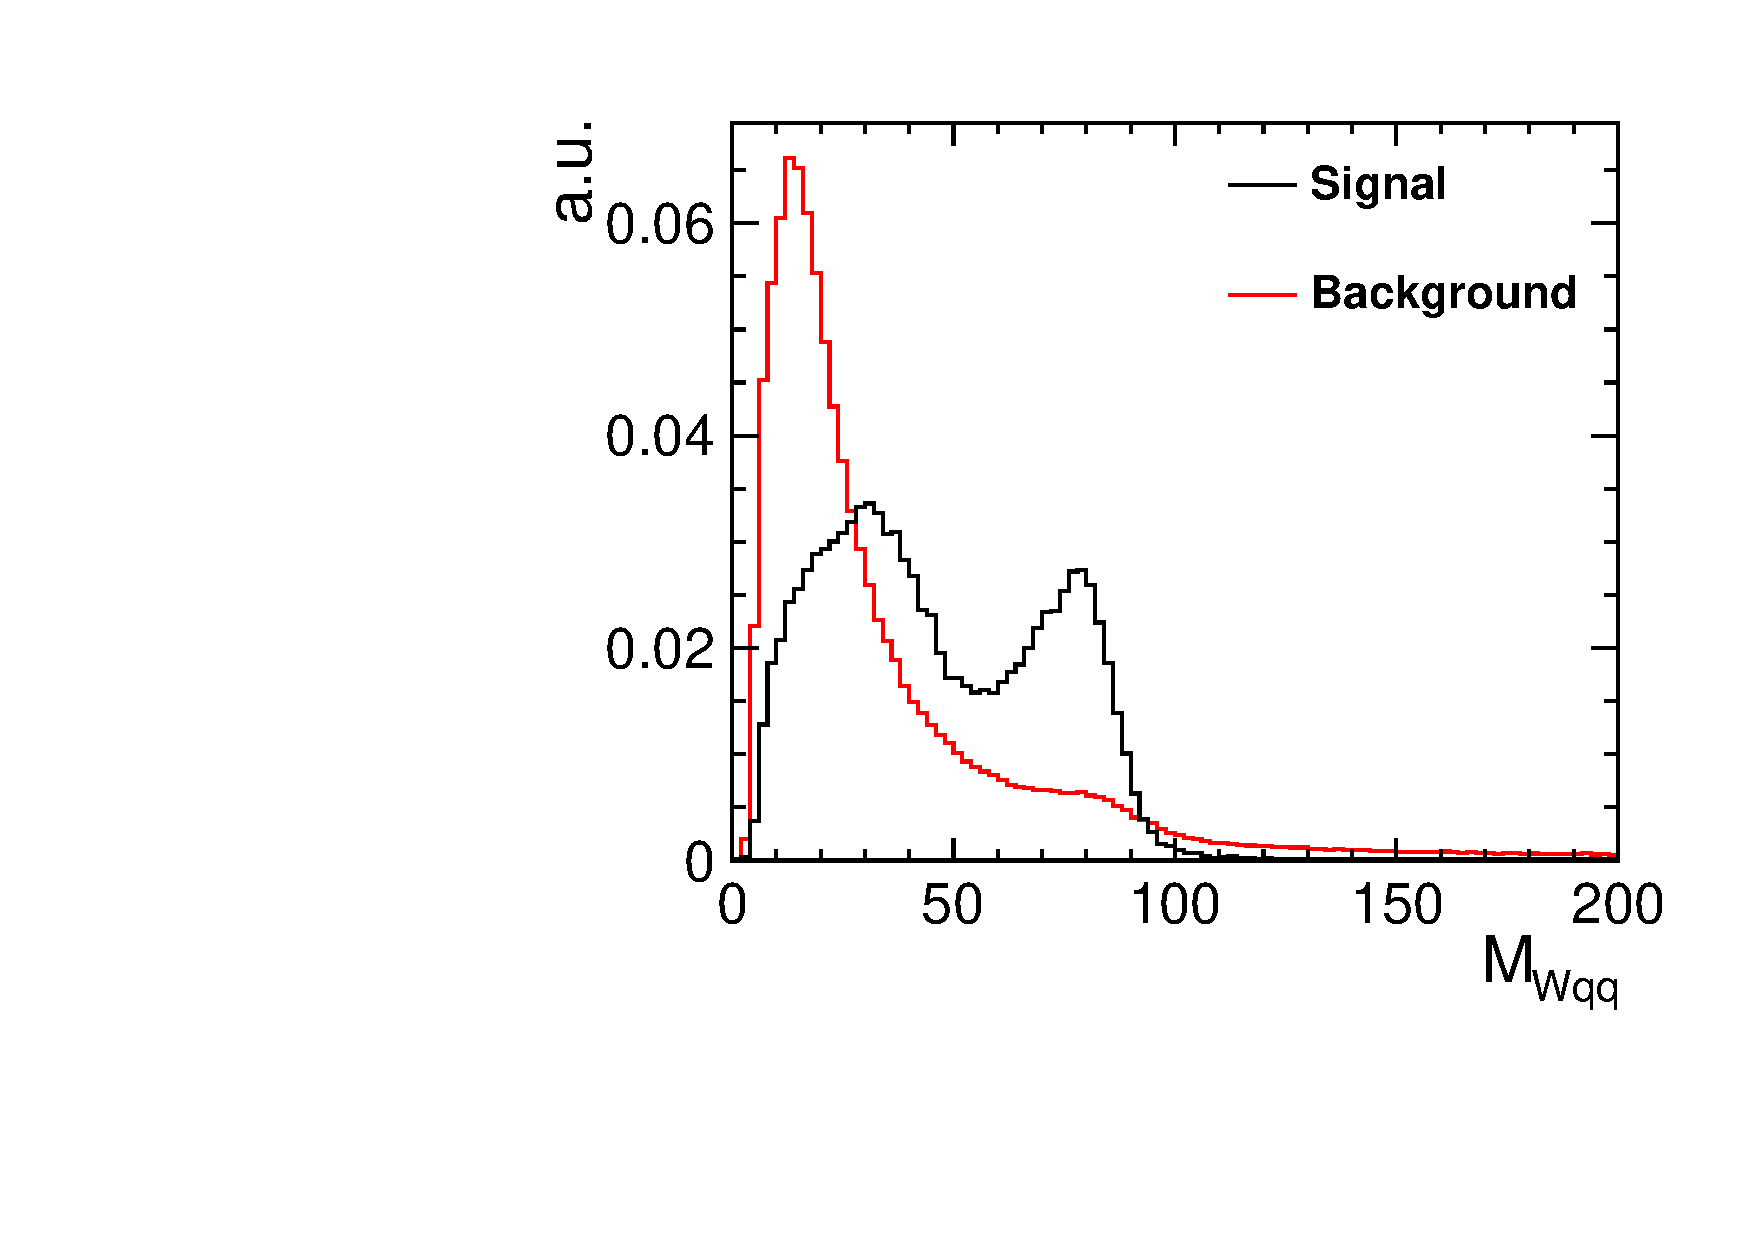
\includegraphics[width=0.75\linewidth]{Appendix/figures/MWqq} 
    \caption{Mass of hadronically decaying W} 
    \vspace{4ex}
  \end{subfigure}%%
  \begin{subfigure}[]{0.5\linewidth}
    \centering
    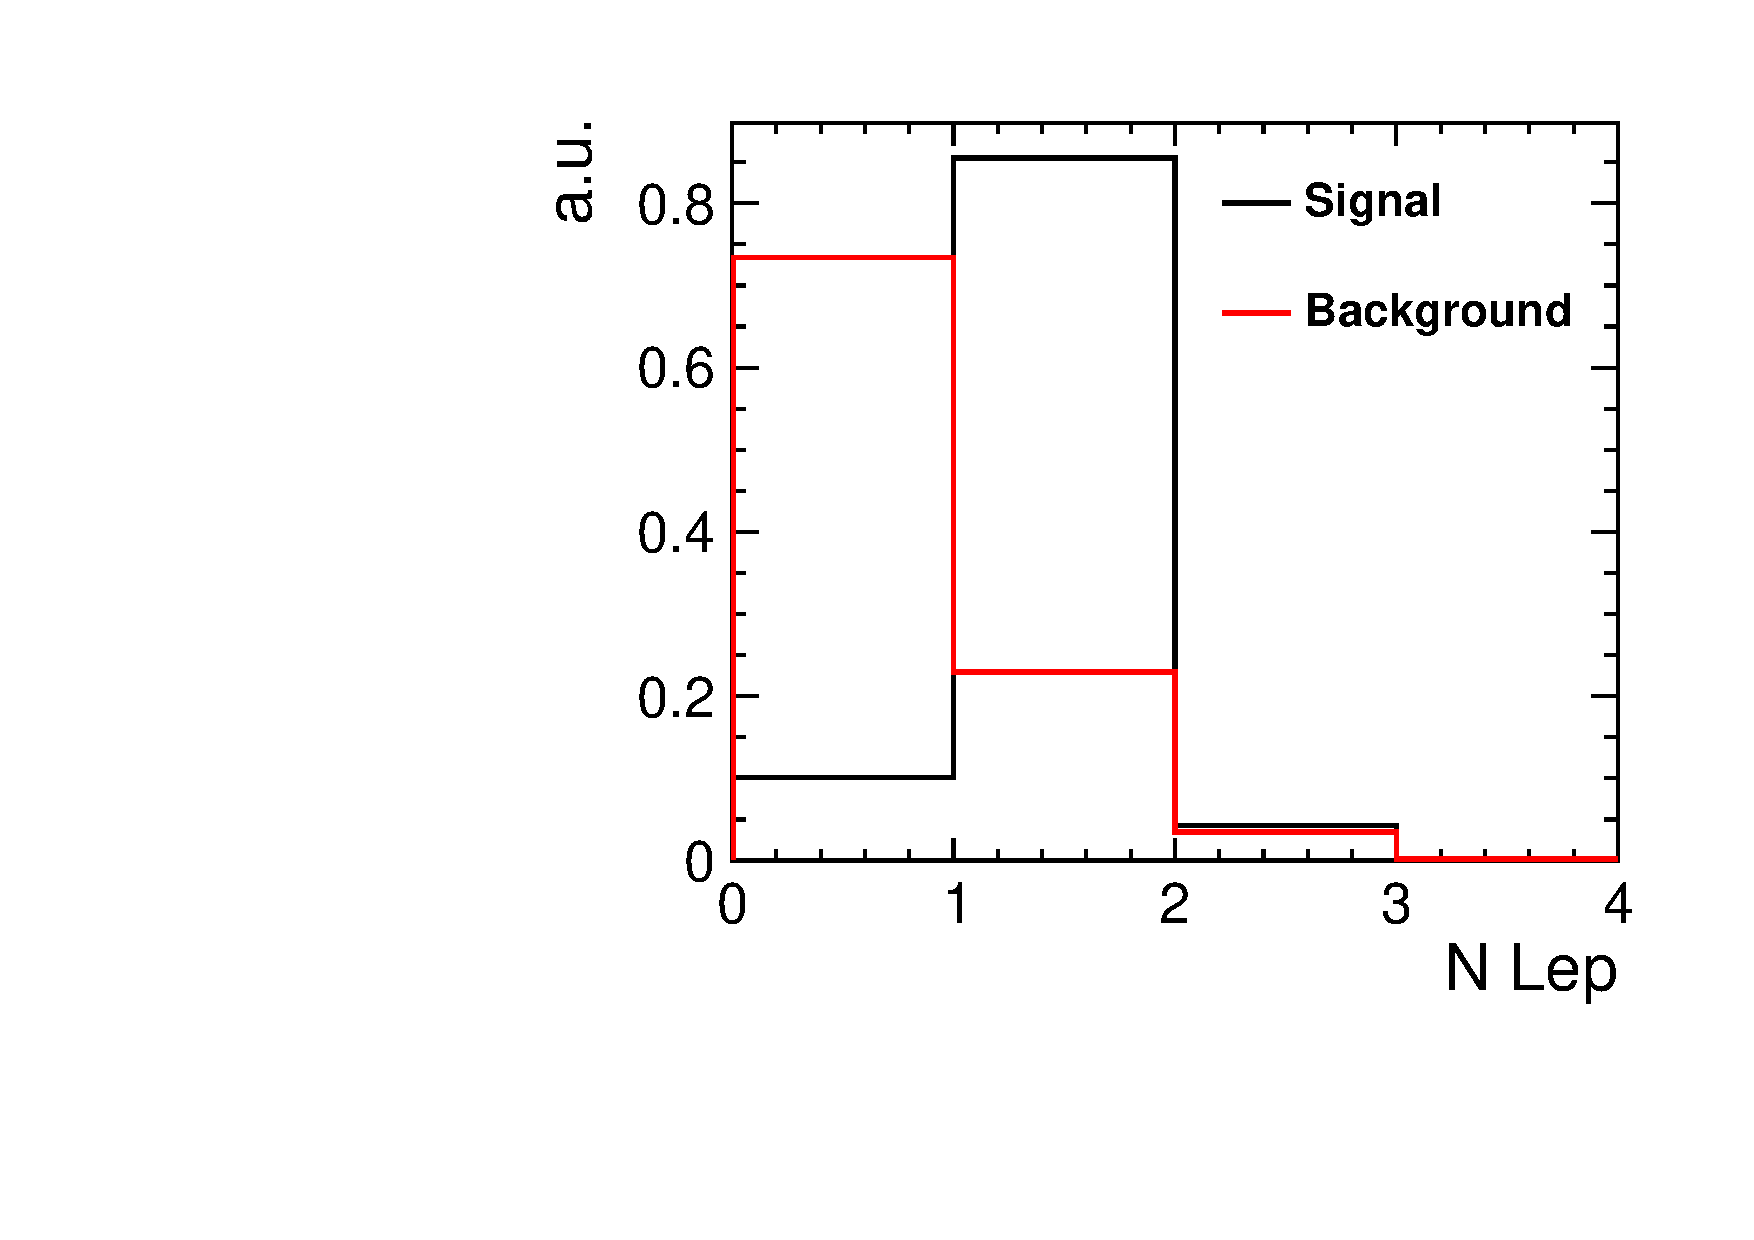
\includegraphics[width=0.75\linewidth]{Appendix/figures/nLep} 
    \caption{Number of reconstructed leptons} 
    \vspace{4ex}
  \end{subfigure}
  \begin{subfigure}[]{0.5\linewidth}
    \centering
    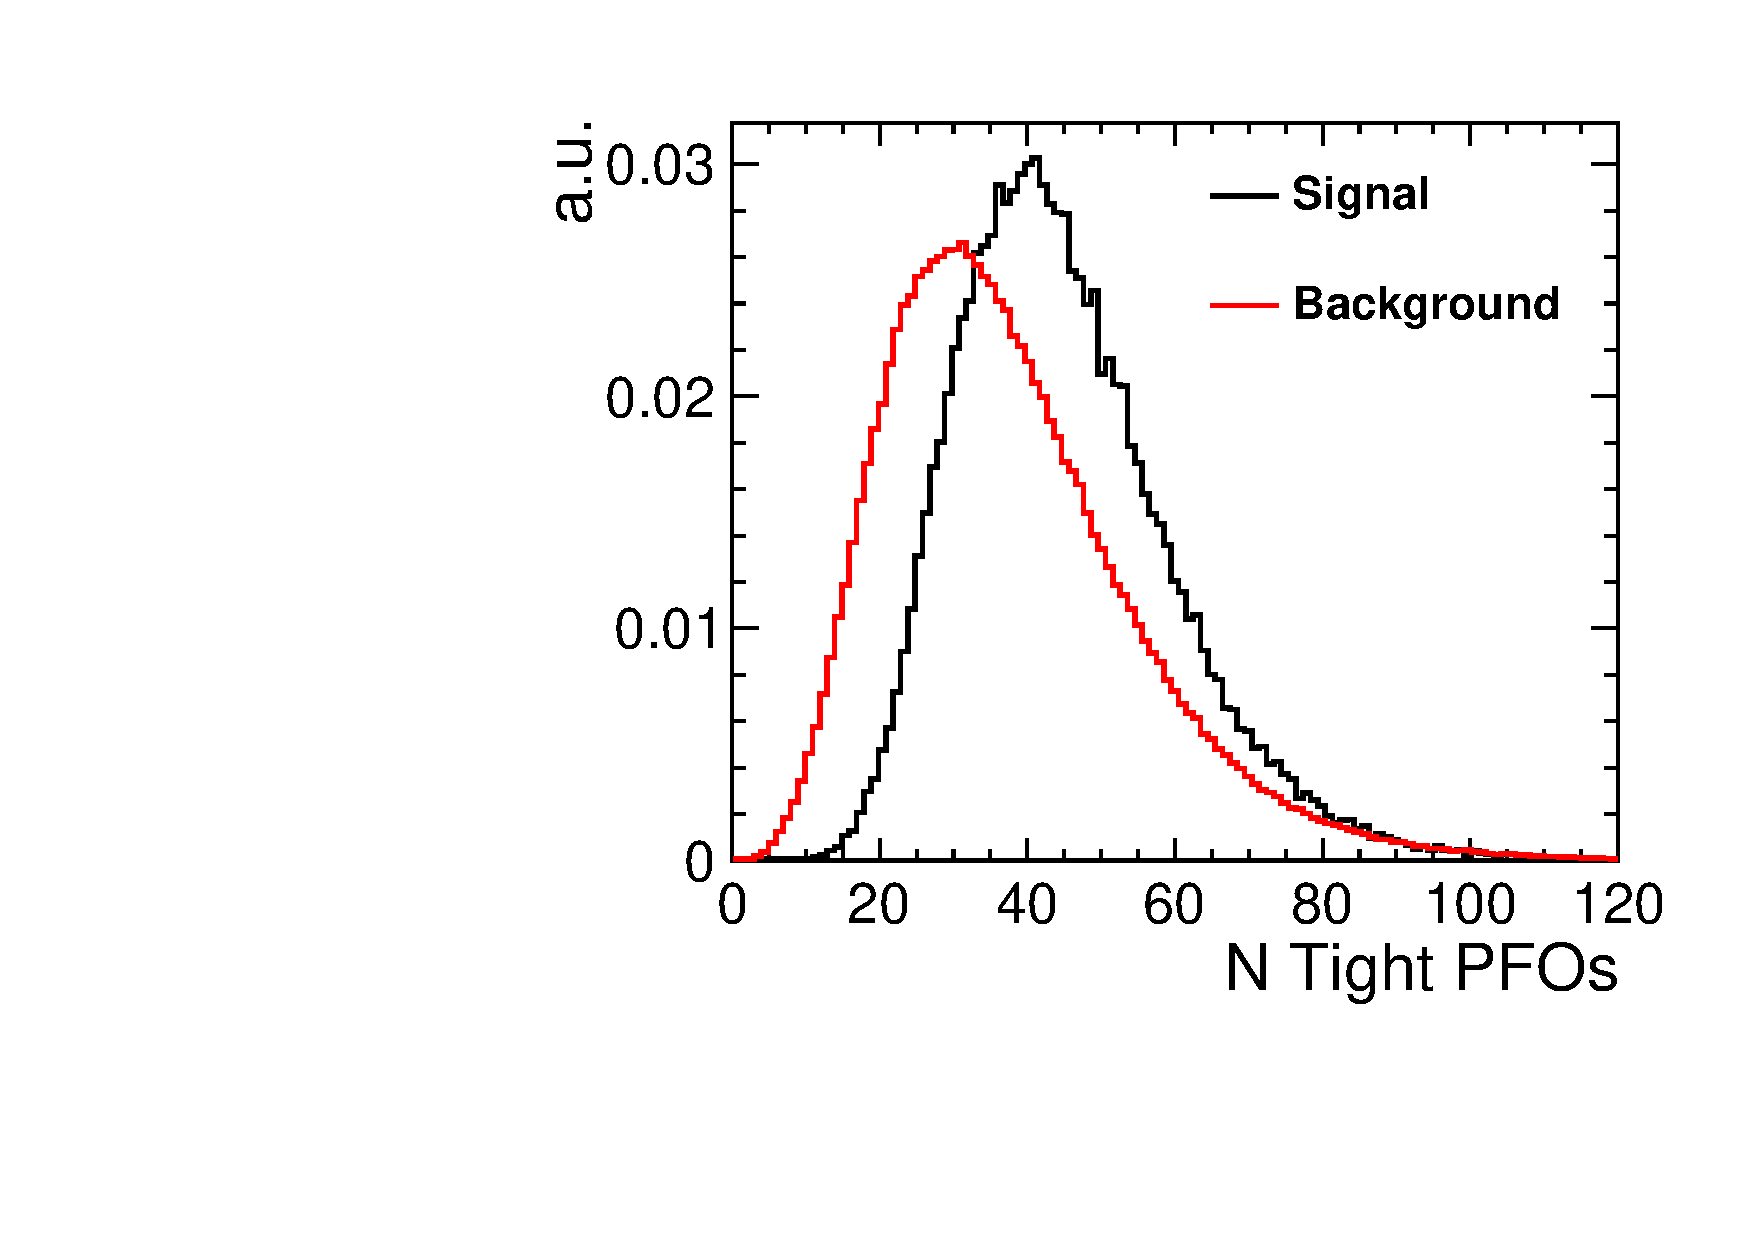
\includegraphics[width=0.75\linewidth]{Appendix/figures/NTightPFOs} 
    \caption{nPFOs passing tight timing cuts} 
    \vspace{4ex}
  \end{subfigure}%% 
  \begin{subfigure}[]{0.5\linewidth}
    \centering
    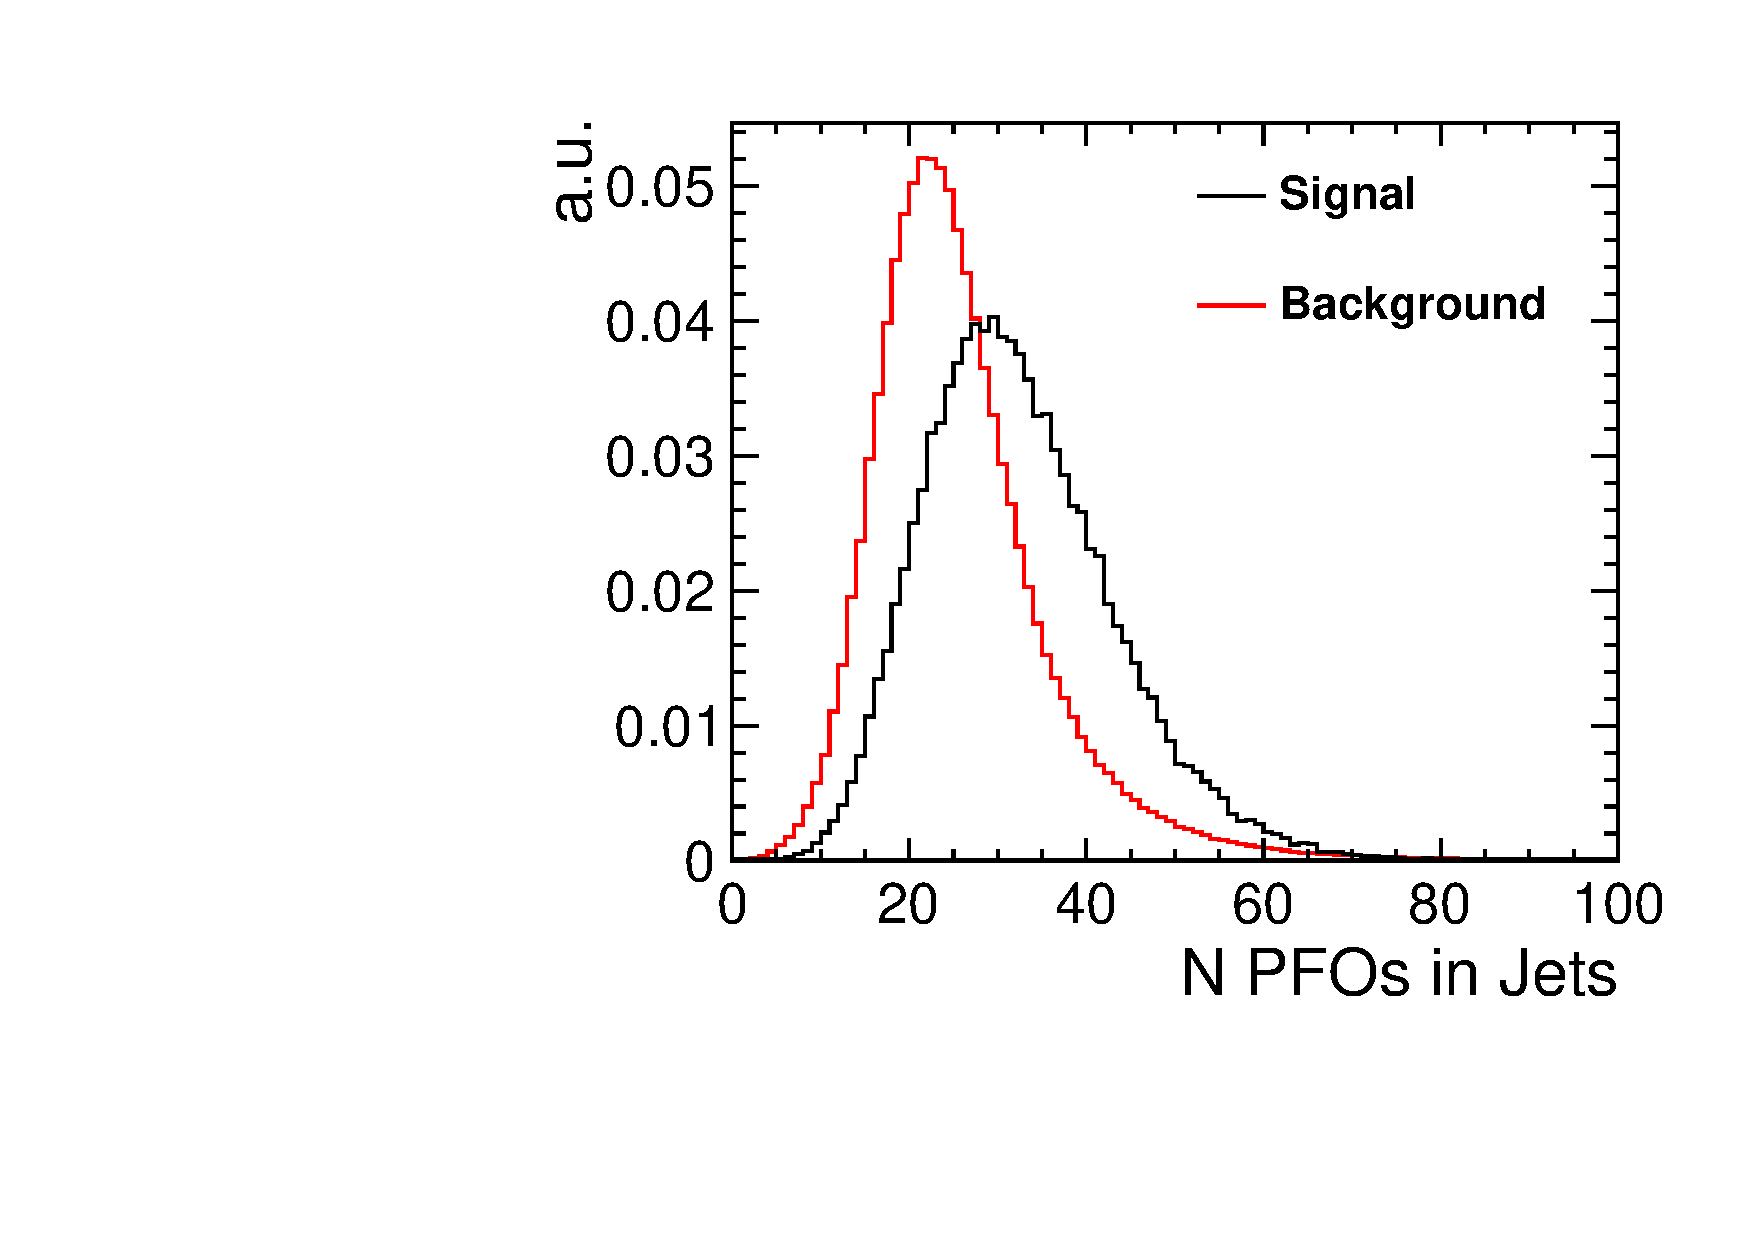
\includegraphics[width=0.75\linewidth]{Appendix/figures/PFOsInJets} 
    \caption{nPFOs assigned to jets} 
    \vspace{4ex}
  \end{subfigure} 
  \begin{subfigure}[]{0.5\linewidth}
    \centering
    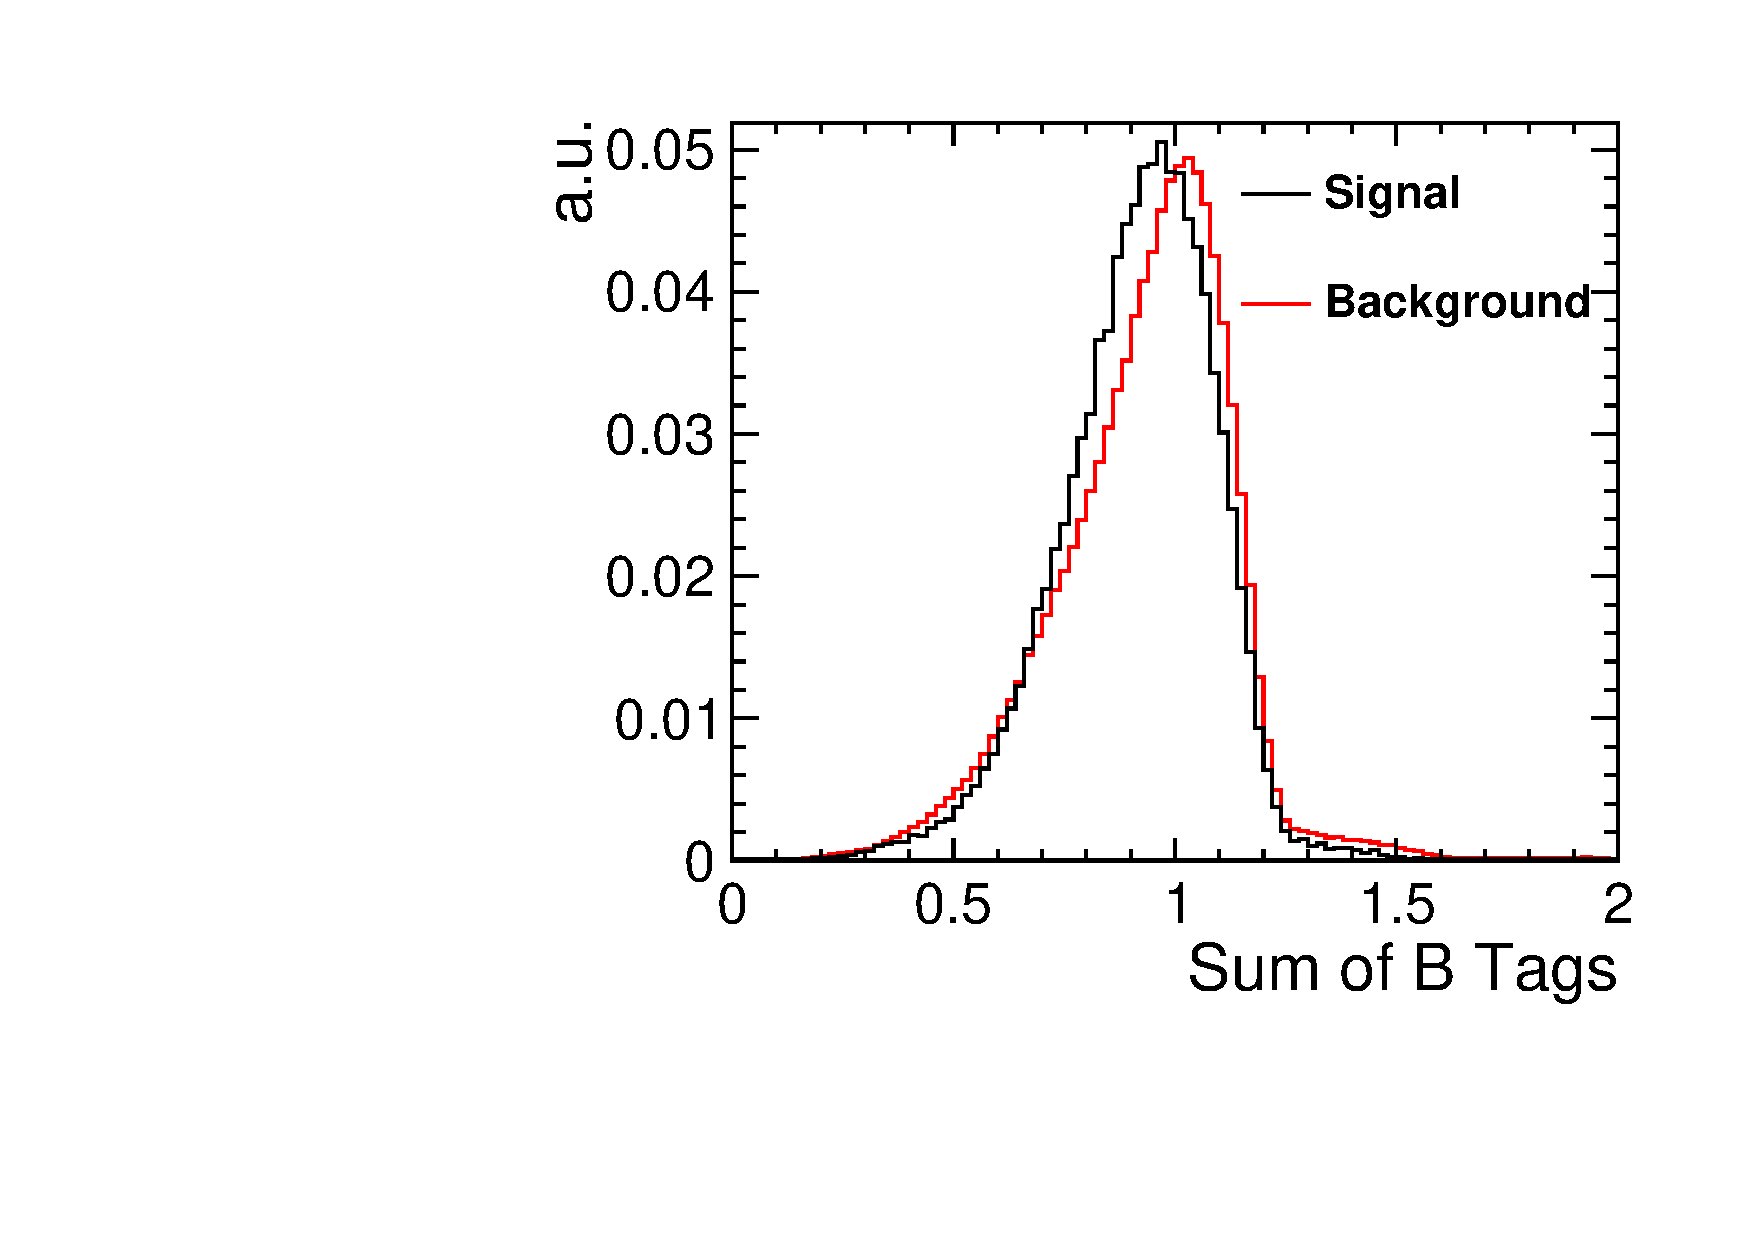
\includegraphics[width=0.75\linewidth]{Appendix/figures/SumBTags} 
    \caption{Sum of two highest b-tags} 
     \vspace{4ex}
 \end{subfigure}%%
  \begin{subfigure}[]{0.5\linewidth}
    \centering
    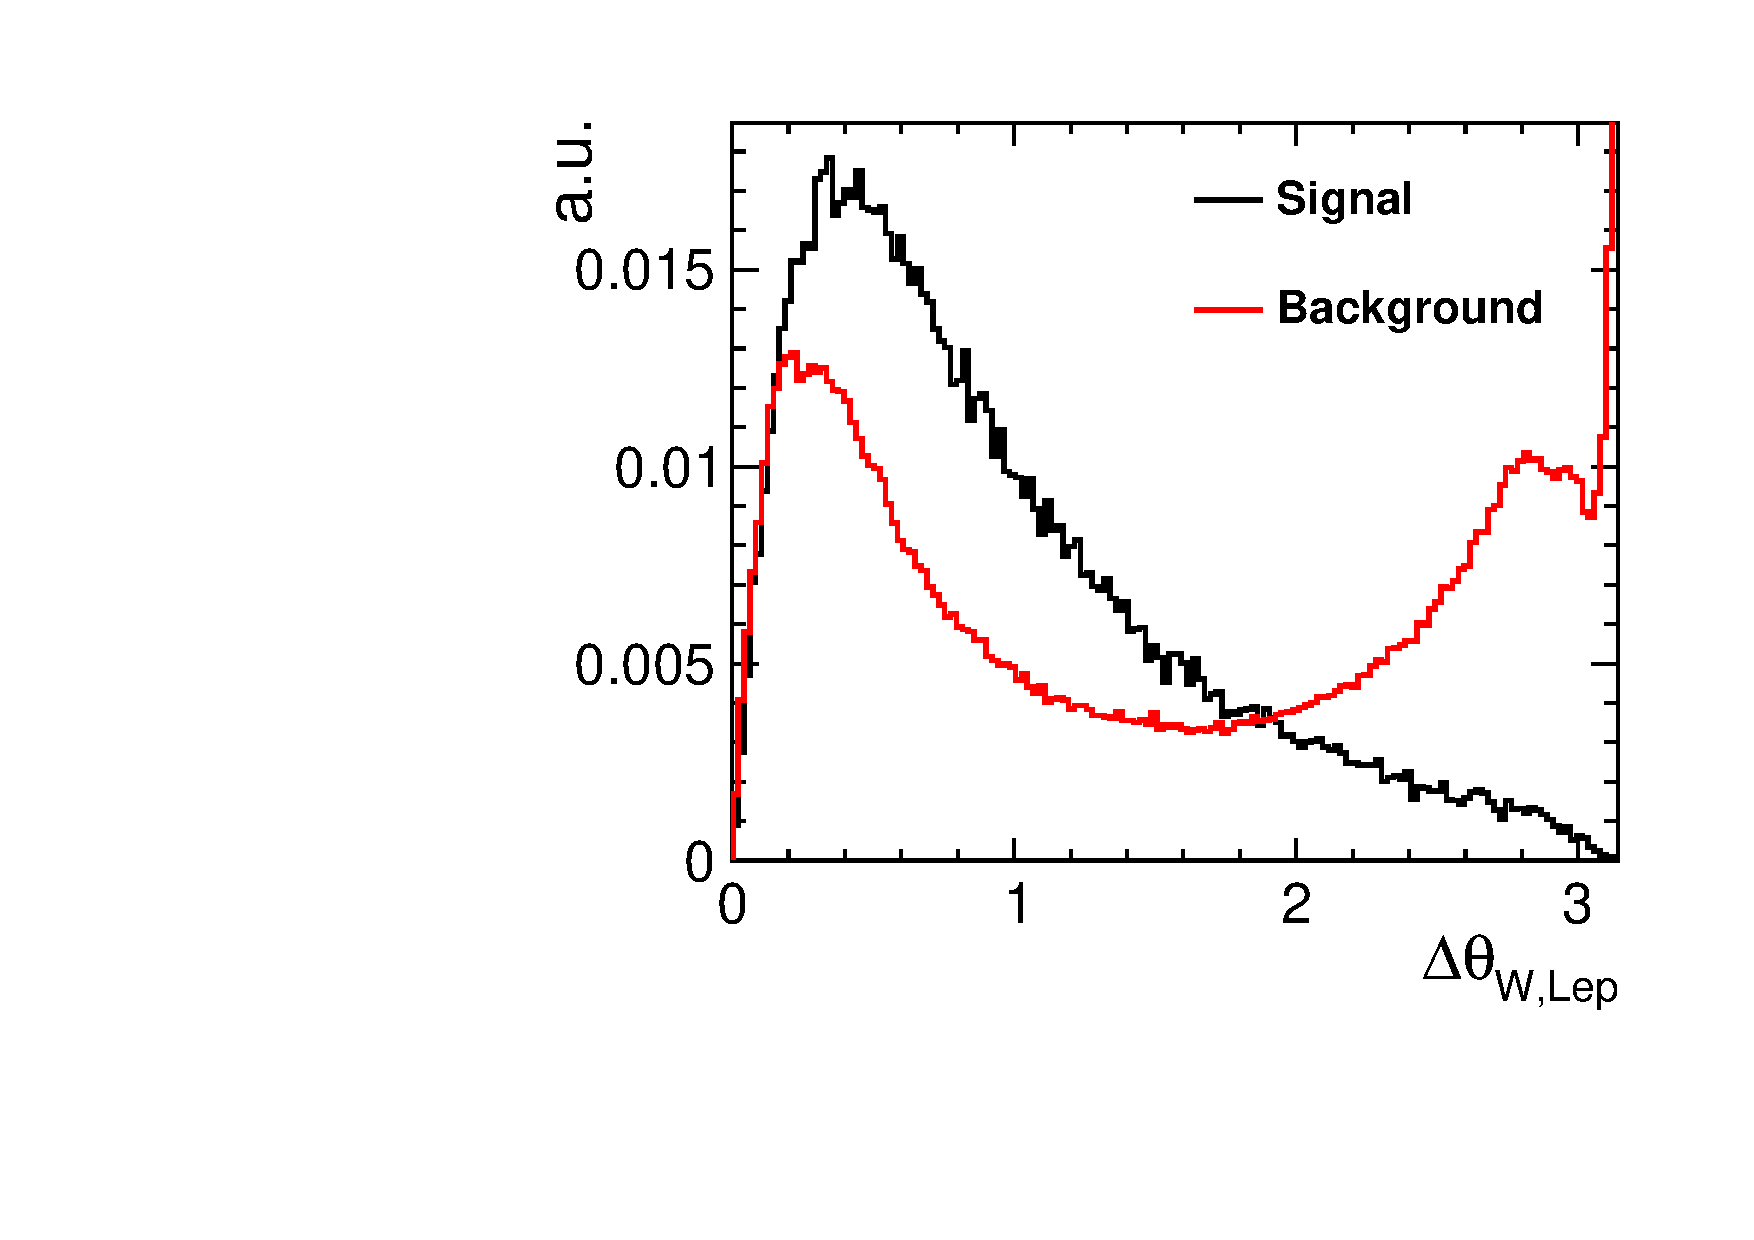
\includegraphics[width=0.75\linewidth]{Appendix/figures/WqqLepAngSep} 
    \caption{Angular Separation of the W and lepton} 
    \vspace{4ex}
  \end{subfigure}
  \begin{subfigure}[]{0.5\linewidth}
    \centering
    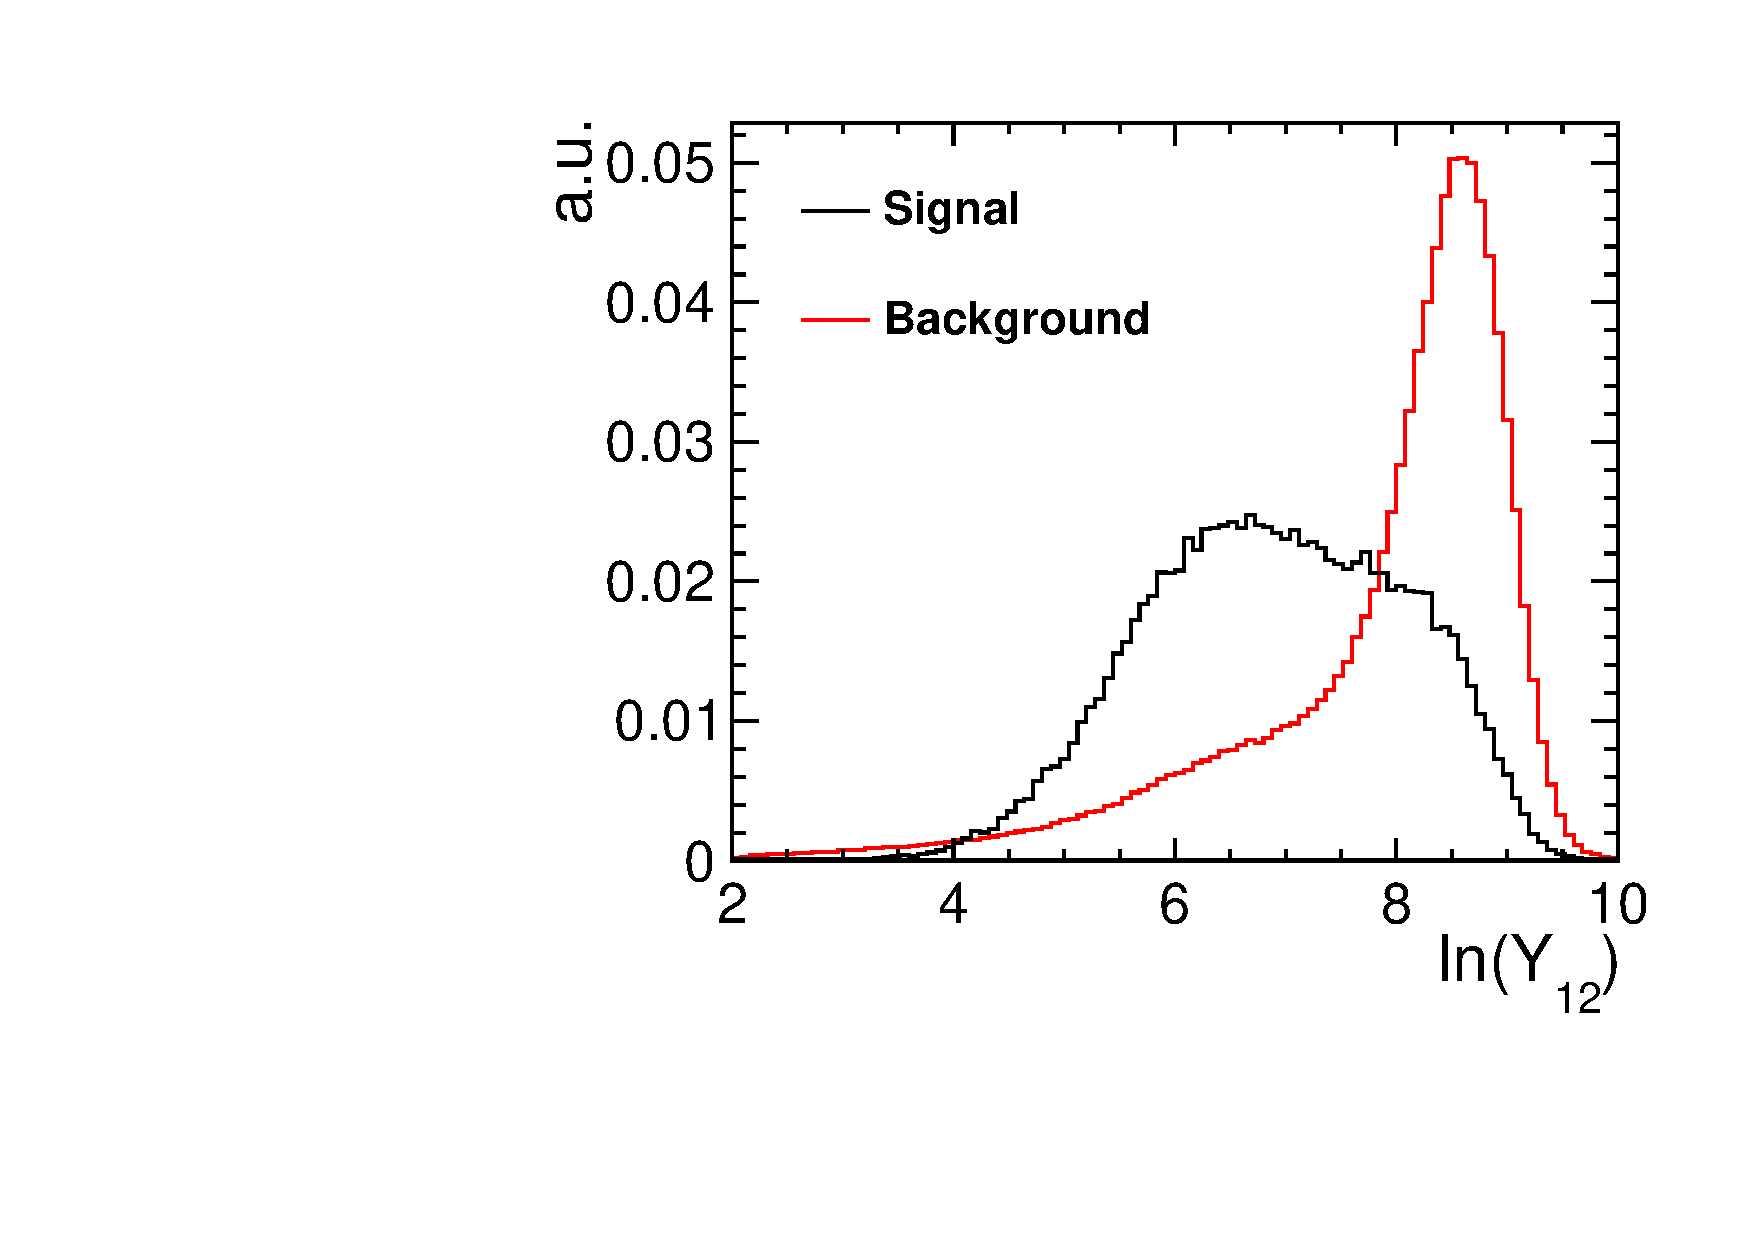
\includegraphics[width=0.75\linewidth]{Appendix/figures/Y12} 
    \caption{Jet Resolution Parameter Y$_{12}$} 
    \vspace{4ex}
  \end{subfigure}%%
\end{figure}

